\chapter{Activity under steady microfluidic flow}
\label{chap:activityAndFlow}

\section{Introduction}
In the previous chapter, we found that when using conditioned media for flow the cultures' viability may be extended so as to allow conducting of useful experiments. The viability assay used, however, is a crude measure of neuronal functionality and indicates that a cell has died only at late stages of apoptosis / necrosis, after the plasma membrane had been breached. This Ph.D work is concerned with how volume transmission interacts with network activity and plasticity so electrophysiological measurements are the relevant measure of functionality. In this chapter, we used multi electrode array electrophysiology to monitor the network activity of the culture as it was subjected to steady microfluidic flow at various flow rates and media formulations. We also explored using a semi-permeable membrane to de-couple the flow from the cells. The media formulation described in the previous chapter as `highly conditioned' was found in preliminary experiments to be inadequate for electrophysiology under flow as it gave rise to inconsistent results and generally to silencing of most of the activity. Thus, the experiments in this chapter are predominantly based on using conditioned media taken from the same culture dish (i.e., media which the particular tested culture grew in, termed `self media') and this approach was the one that finally gave usable behaviour. Nevertheless, how flowing with media from other culture dishes affects the activity was also explored.

We found a strong flow rate dependent effect whereby for slow flow rates the network dynamics were preserved. For faster flow rates, a disruption to the network activity was observed consisting a partial silencing of the active MEA channels and a loss of synchronization and of the response to electrical stimulation. This disruption was present even when a semi-permeable membrane was used to de-couple the cells from the flow. Such a membrane was shown to reduce the shear underneath to negligible levels \cite{morel2012concentration} so this observation strongly suggests that the cause of the effect is a disturbance to the chemistry around the cells. An improvement in the stability of activity was provided by the use of media from older cultures but this was still inconsistent. Finally, we found that typical synchronized network dynamics were preserved in older cultures (aged over 20 days \textit{in vitro}) under fast flow but this was still strongly dependent on the source of the media (self media vs. media from younger culture).  We argue that these results indicate an interaction between the flow and intrinsic volume transmission signalling in the tissue and propose that microfluidic flow could potentially be used as a novel assay to study these poorly understood processes. Furthermore, these results highlight the important factors that need to be addressed when designing microfluidic based drug delivery systems to neuronal tissue and the implications for device design are discussed. Most importantly, This study provides a protocol where network activity is preserved under rapid flow and is therefore the basis for the final microculture pulsing system presented in chapter \ref{chap:microculturePulses}.

\label{sec:crossFlow:intro}

\section{Neuronal cultures in cross flow devices on MEAs}
Figure \ref{fig:crossFlow:crossFlowIllustration} shows the devices used for the experiments conducted in this chapter. In contrast to the devices used for the viability study in chapter \ref{chap:devicesAndFlow}, these devices comprised multiple layers so as to allow the inclusion of the semi-permeable membrane (Whatman cyclopore, \(100 nm\) pore size, cat. no. 7060-4701). Thus they comprised a flow and cell layers which were joined either to each other or to the membrane from each side, depending on the experiment. Because of the perpendicular arrangement of the flow channel in relation to the cell channel the devices were tagged `cross flow'. Since assembly of such multi layered devices through plasma bonding is problematic and since plasma bonding of PDMS to the commercial MEAs could damage the surface and is not practical for re-use, we opted to use the tape technology (section \ref{sec:devices:bonding}). Thus prior to device placement, the MEA surfaces were treated with PEI (section \ref{sec:methods:surface}). In parallel, the device layers were cut out of the \(125 \mu m\) silicone transfer tape and aligned using a custom made alignment tool (essentially comprising two pegs holding the layers in place through alignment ports). The assembled devices were oven sterilized and joined with the MEA surfaces, after these have been washed and dried from the PEI solution. The devices were manually aligned to the MEAs in such a way that the intersection area between the flow and cell channels was on top of the central electrode pads area. Since self media is extracted directly from the tested sample we increased the volume of growth media to \(4 ml\) per sample to make sure that enough supply would be available for the flow session. We used custom made glass cylinders which were glued to the MEA following the attachment of the devices to hold the media (figure \ref{fig:pulses:circularIllustration}).

 \begin{figure}[h]
       \centering
       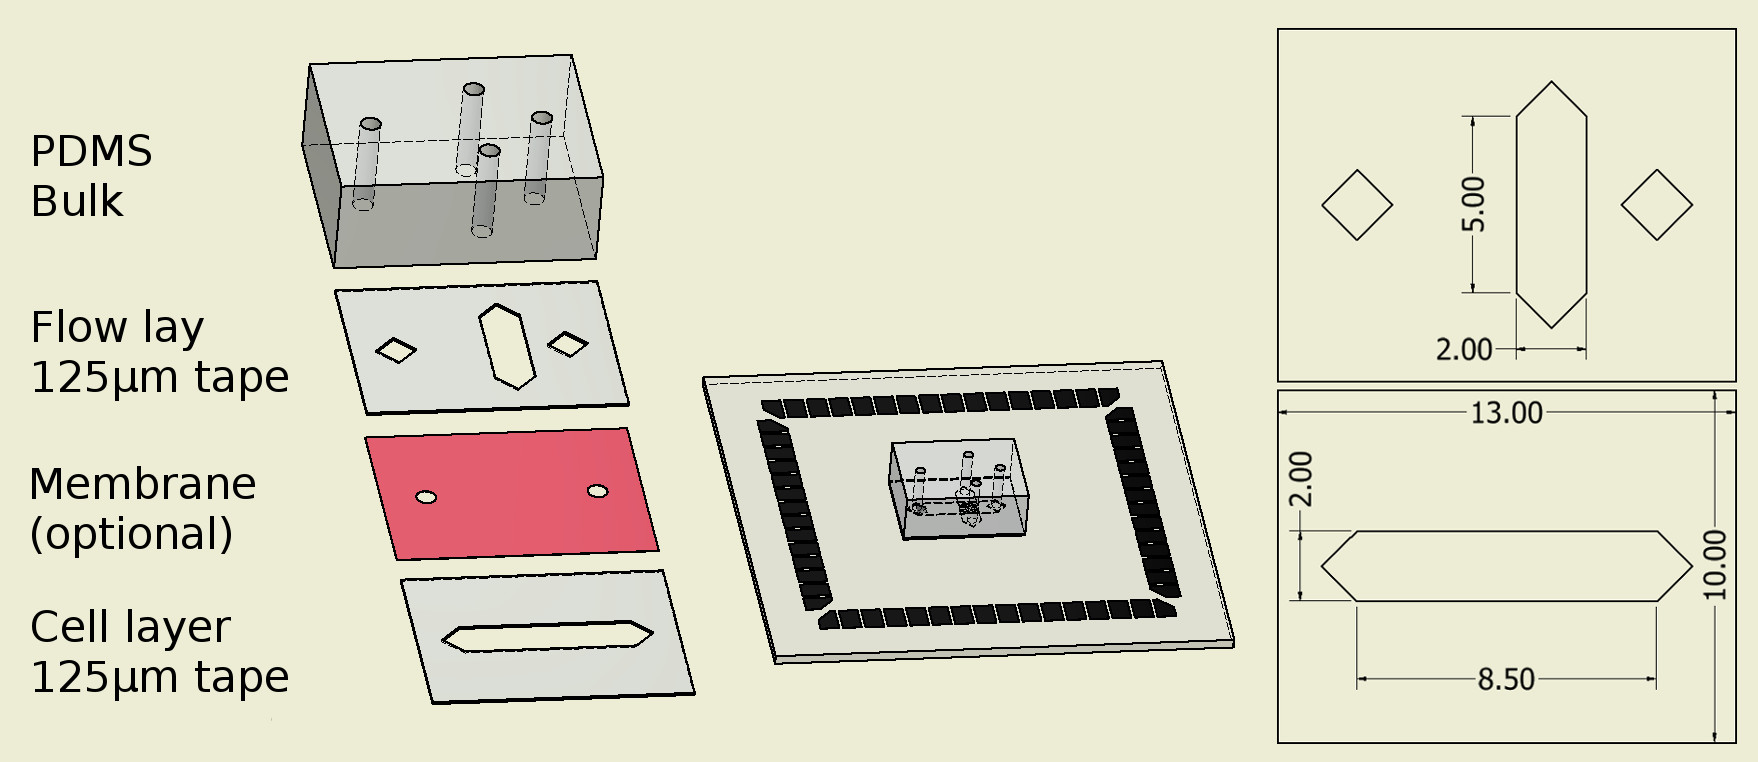
\includegraphics[width=15cm]{chapter5/figures/crossFlowIllustration/crossFlowIllustration.jpg}
       \caption[Illustration of the cross flow devices used for measuring culture activity under flow]{\textbf{Illistration of the cross flow devices.} Illustrations showing the constituent layers of the device laid out as well as assembled and joined to an MEA. The semi-permeable membrane is optional and shown in red. The dimensions of the flow and cell layers are also shown in millimeter units. Further details about the device fabrication are found in the text.}
       \label{fig:crossFlow:crossFlowIllustration}
  \end{figure}

To seed the cross flow devices, the flow channel ports were blocked so as to prevent seeding solution from being diverted through the flow channel. The seeding volume was \(3 \mu L\) which is enough to fully saturate the cell layer (\(\approx 2 \mu L\)). The seeding density was \(7\times 10^6\frac{cells}{ml}\) which was calibrated to achieve an area density of \(\approx 1000 \frac{cells}{mm^2}\) in the central electrode pads area. Cultures seeded in such devices typically developed well for over a month. This contrasted with the standard 1-layered devices introduced in section \ref{sec:devices:protocolDev} where many of the cultures did not develop past the end of the 3\textsuperscript{rd} week. This could be attributed to the increased volume of the cross flow devices which would be associated with improved nutrient and by product circulation or to the switch to PEI surface treatment which is considered better for neuronal adhesion. Maintenance of the seeded devices was as described in \ref{sec:methods:culture} and completely follows the protocol achieved in section \ref{sec:devices:protocolDev}.



  \begin{figure}[!htb]
       \centering
       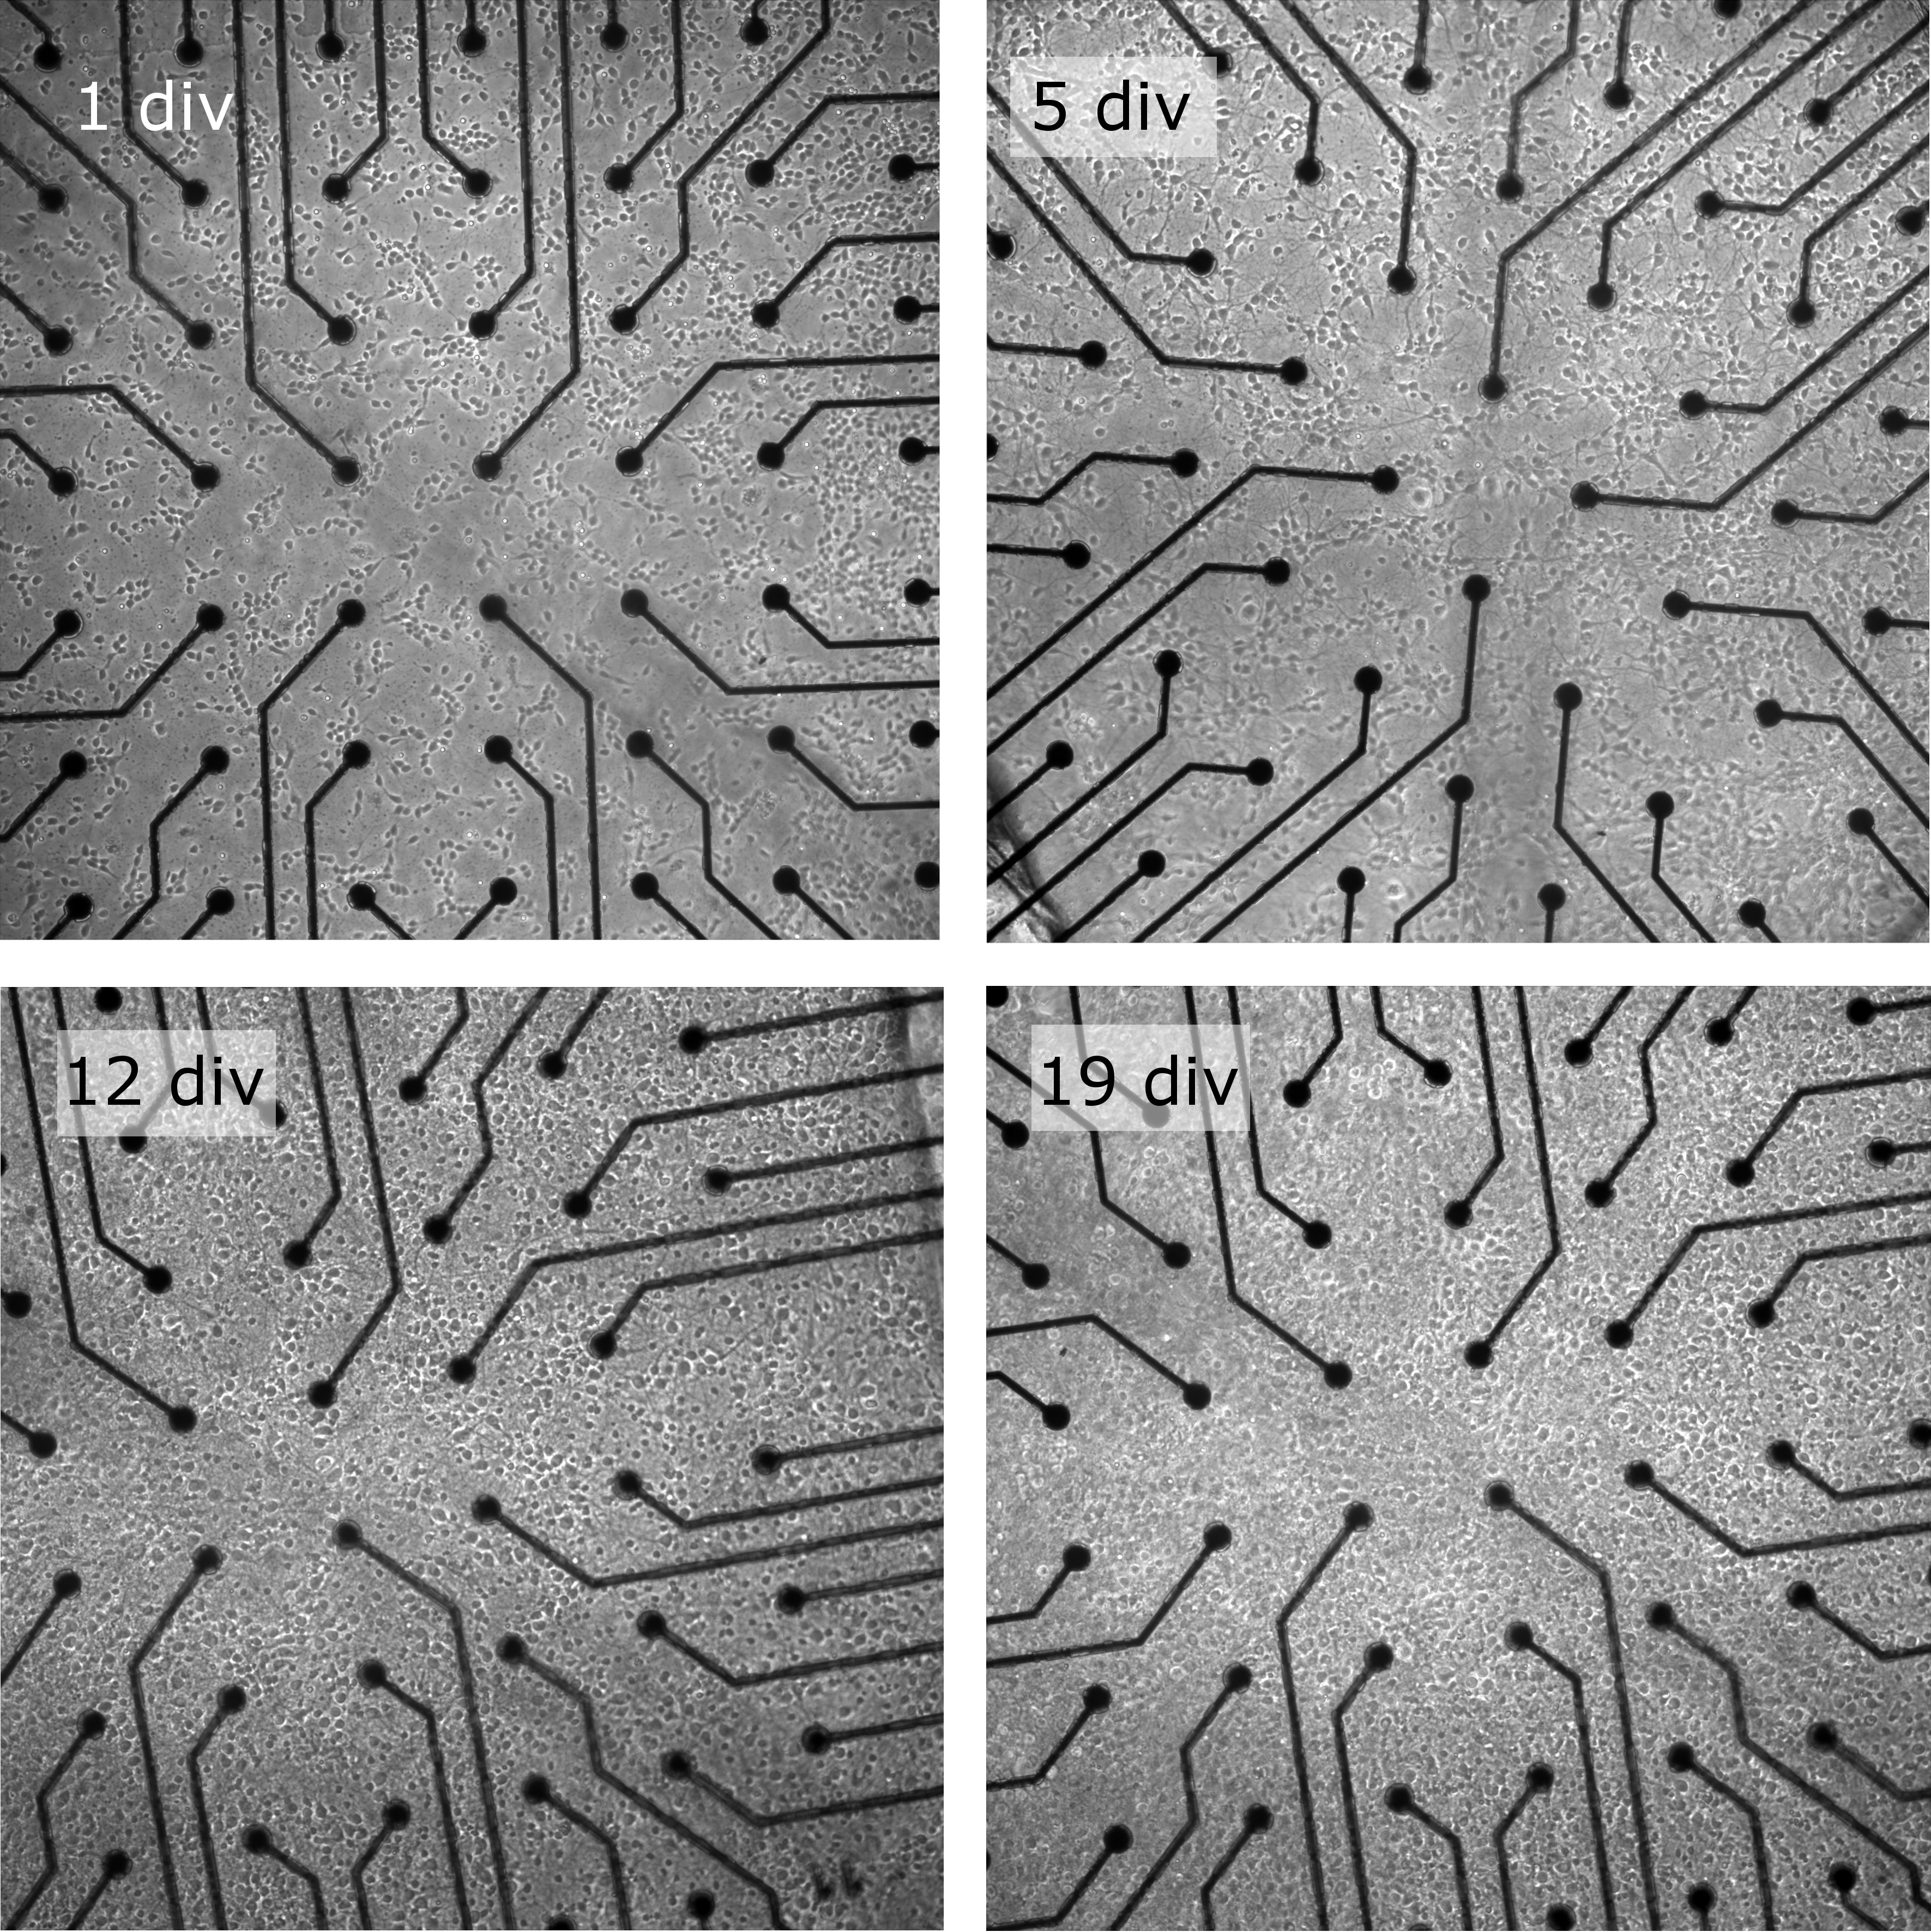
\includegraphics[width=15cm]{chapter5/figures/crossFlowDev/culture.jpg}
       \caption[Images of a neuronal culture growing in cross flow devices]{\textbf{Neuronal cultures develop well in cross flow devices for over 3 weeks \textit{in vitro}.} Images of neuronal culture growing in the cross flow devices at several developmental time points. The images were taken in the area of intersection between the flow and cell channels. The electrodes are spaced \(200 \mu m\) apart for length reference.}
       \label{fig:crossFlow:crossFlowDev}
  \end{figure}


\section{Activity under flow for young cultures}
        The first set of experiments were performed on cultures at ages 12-15 days \textit{in vitro} which were termed `young' cultures. This age range is similar to the one used for the viability study in section \ref{sec:devices:viability} so the results shown here probably best reflect the state of the cultures in that study. The recordings in this chapter were all performed in the presence of electrical stimulation in the form of a single test pulse delivered to a single MEA electrode every 5 seconds. The stimulating electrode and the pulse voltage amplitude were selected before the experiment so that an observable network response would be elicited by the stimulation. The reason for using stimulations is twofold: firstly, spontaneous activity is known to be inherently volatile as it probably depends on stochastic processes of intrinsic excitability and synaptic noise. Since the aim of these experiments is to identify conditions where the activity is stable we were concerned that variability associated with spontaneous activity would be confused with the destabilizing effects of flow. Thus, we argued that electrical stimulation which is more deterministic than spontaneous activity might be a more adequate basis for assessing the stability under flow. Secondly, the ability of neuronal ensembles to respond to stimulation underlies their facility for representing and transforming external information. We therefore found it is important to include a criteria where the response to stimulation would be maintained under flow.

        The extracellular recordings and data analysis pipeline as well as the stimulation protocol are specified in section \ref{sec:methods:MEARecording} and have been further described in sections \ref{sec:activity:spontActivity} and \ref{sec:activity:evoked}. All the experiments described in this chapter were initiated with a 30-60 minute period of baseline recording before the sample was plugged into the flow system. When self media was used, it was withdrawn from the sample and flushed through the system after the baseline recording.

        \subsection{Effect of flow rate}
        \label{sec:crossFlow:slowFast}
        We found a strong flow rate dependent effect on the activity which is exemplified in figure \ref{fig:crossFlow:slowFastExample} which shows baseline as well as slow and fast flow data for a young culture. In the baseline recording, the culture exhibited typical synchronized bursting dynamics which are typical for rat cultures of this age (sections \ref{sec:activity:spontActivity} and \ref{sec:activity:mouseRatComp}). These synchronized dynamics were manifested in vertical lines in the raster plots and with high values of correlation throughout the correlation matrix. Additionally, the culture responded to test stimulation pulses with a network reverberation, although these sometimes failed to appear. Immediately upon initiation of the fast flow, these synchronized dynamics broke down with the neurons initially switching to a fast tonic firing and then gradually becoming silent. The tonic firing was manifested in a dramatic reduction in the correlation values. Additionally, the stimulation response was all but completely abolished with the activity not occurring preferentially after the stimulation but tonically spread in the observed time window (figure \ref{fig:crossFlow:slowFastExample} B). Remarkably, even the direct responses (low latency, low jitter responses appearing as straight lines in the response rasters) were abolished under flow which suggests that the basic biophysics of the neurons had been compromised. Under slow flow, there was no sign of these dramatic perturbations to the activity. Indeed, it is evident that the slow flow induced some changes to the activity but overall the synchronized bursting dynamics and the stimulation responses were maintained and the structure of the correlation matrix was preserved.

        \begin{figure}[!htb]
            \centering
            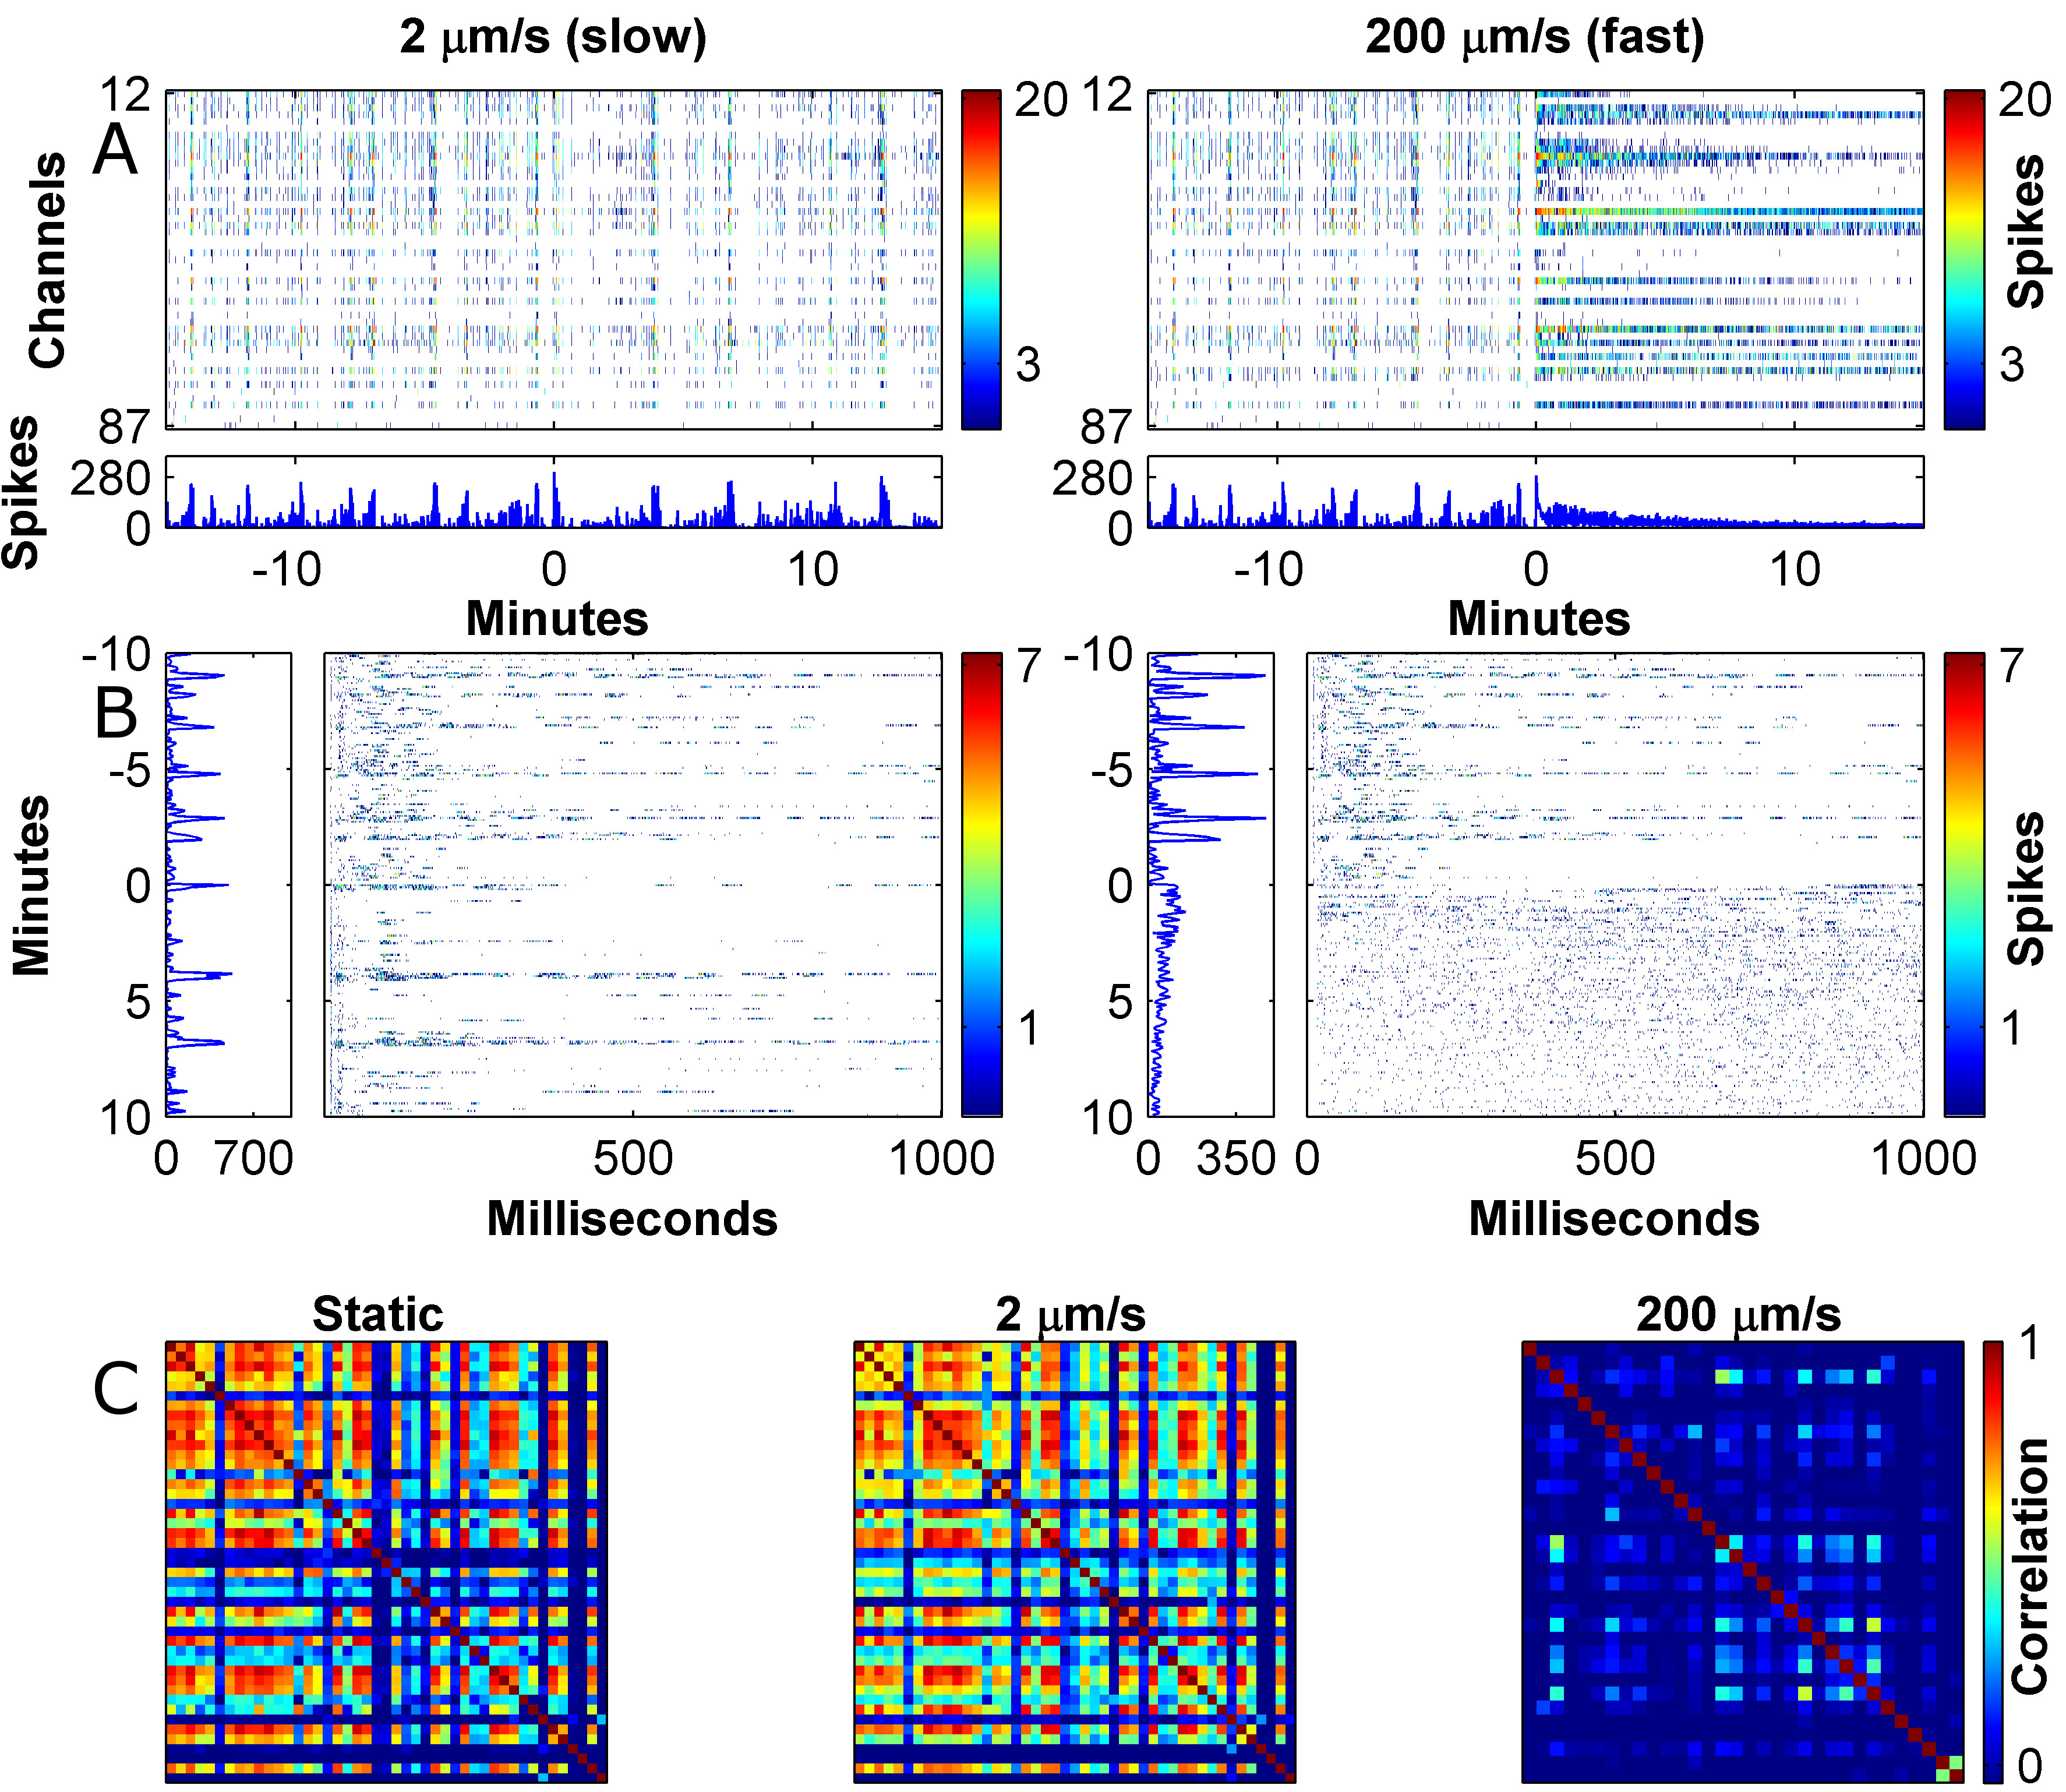
\includegraphics[width=15cm]{chapter5/figures/slowFastExample/slowFastExample.jpg}
            \caption[Example for the Effect of flow rate on the activity of a young culture under flow]{\textbf{Young cultures placed under flow with self media suffer a flow rate dependent disruption to the activity.} (A) Network raster plots showing the activity of the culture before (negative times) and just after (positive times) initiation of slow and fast flow (left and right panels, respectively). Note the immediate switch to a tonic and desynchronized regime in the case of the fast flow (B) The culture's network responses to stimulation before and just after initiation of slow and fast flow. Note the immediate loss of the temporally localized stimulation response in the case of fast flow (C) Correlation matrices representing the culture's activity in static conditions and under flow. All matrices are based on 10 minute activity samples. In the case of flow the samples were taken 15 minutes into the flow session. To obtain the shown data, the culture was initially recorded for 30 minutes in baseline conditions following which the flow tubes were connected and 20 minutes of slow flow were recorded. The flow was then increased to the fast rate and remainder of the session was recorded in this setting. This experimental sequence was an exception which was made to observe different flow rates applied to the same culture. In the typical case (figure \ref{fig:crossFlow:slowFastStats}) slow and fast flow regimes were conducted in separate experimental sessions.}
            \label{fig:crossFlow:slowFastExample}
        \end{figure}

        To make sure that the phenomena reported above were indeed consistent we ran several such experiments with slow and fast flow rates and show the statistics in figure \ref{fig:crossFlow:slowFastStats}. The results are presented through 3 measures: global firing rate (i.e, total number of spikes recorded over all electrodes), mean correlation (i.e., the mean of the correlation matrix without the diagonal elements) and stimulation response ratio which is explained next. Stimulation response ratio refers to the ratio between the total spike count (over all electrodes) in a \(200 ms\) window just following the stimulation and a window of the same size 2 seconds later. The reason for this definition is that a measure that counts only the spikes following the stimulation is very sensitive to the background spontaneous activity. Thus we employed a second window at a distance from the stimulation under the assumption that its spike count is attributed solely to spontaneous activity. The ratio measure therefore represents the relative increase in  firing rate due to the stimulation relative to the ongoing spontaneous activity. As some of the conditions used here caused large changes in intensity and temporal distribution of the spontaneous activity, using a simple stimulation response measure would have been meaningless. The firing rate and stimulation response ratios are further normalized to the baseline values of these measures (i.e., from the baseline recording period prior to connection of the tubes). Measures for control cultures were normalized to the mean value over the first hours of recording.

        The above-mentioned activity measures are shown in a brief 40 minute window following flow initiation (figure \ref{fig:crossFlow:slowFastStats} A-C) to observe the immediate consequences and also for an extended period of over 3 hours (figure \ref{fig:crossFlow:slowFastStats} D-E) to assess the longer term behaviour. The short term window was also used for statistical testing. Cultures placed under fast flow with self media showed a rapid reduction in firing rates and synchronicity and their response to stimulation was immediately abolished (difference from control was verified through 2-way ANOVA with \(p=0.005\), \(5\times 10^{-10}\) and \(3\times 10^{-9}\), respectively. P values shown are the lower between the group and the interaction effect). Cultures under fast flow were not able to recover their activity and all the measures tended to zero in the long run. Cultures placed under slow flow did not show a significant difference in firing rate or in stimulation response and had just a marginal decrease in correlation (2-way ANOVA, \(p=0.61\), \(0.20\) and \(0.04\), respectively). It is evident from the long term plots for the firing rate and correlation that there was a high degree of variability associated with the initiation of slow flow (connecting the tubes probably causes a sudden flush of media internally in the device). However, over time the cultures were able to adapt to the conditions and the variability subsided. In the case of the response to stimulation, a dramatic increase was observed from about the 3\textsuperscript{rd} hour of the flow session. This later effect shows that even the slow flow induces changes and instability to the culture over time. However, the mechanism behind this non-trivial effect is probably different from those operating immediately at the onset of flow and was not investigated further in this work.

        \begin{figure}[!htb]
            \centering
            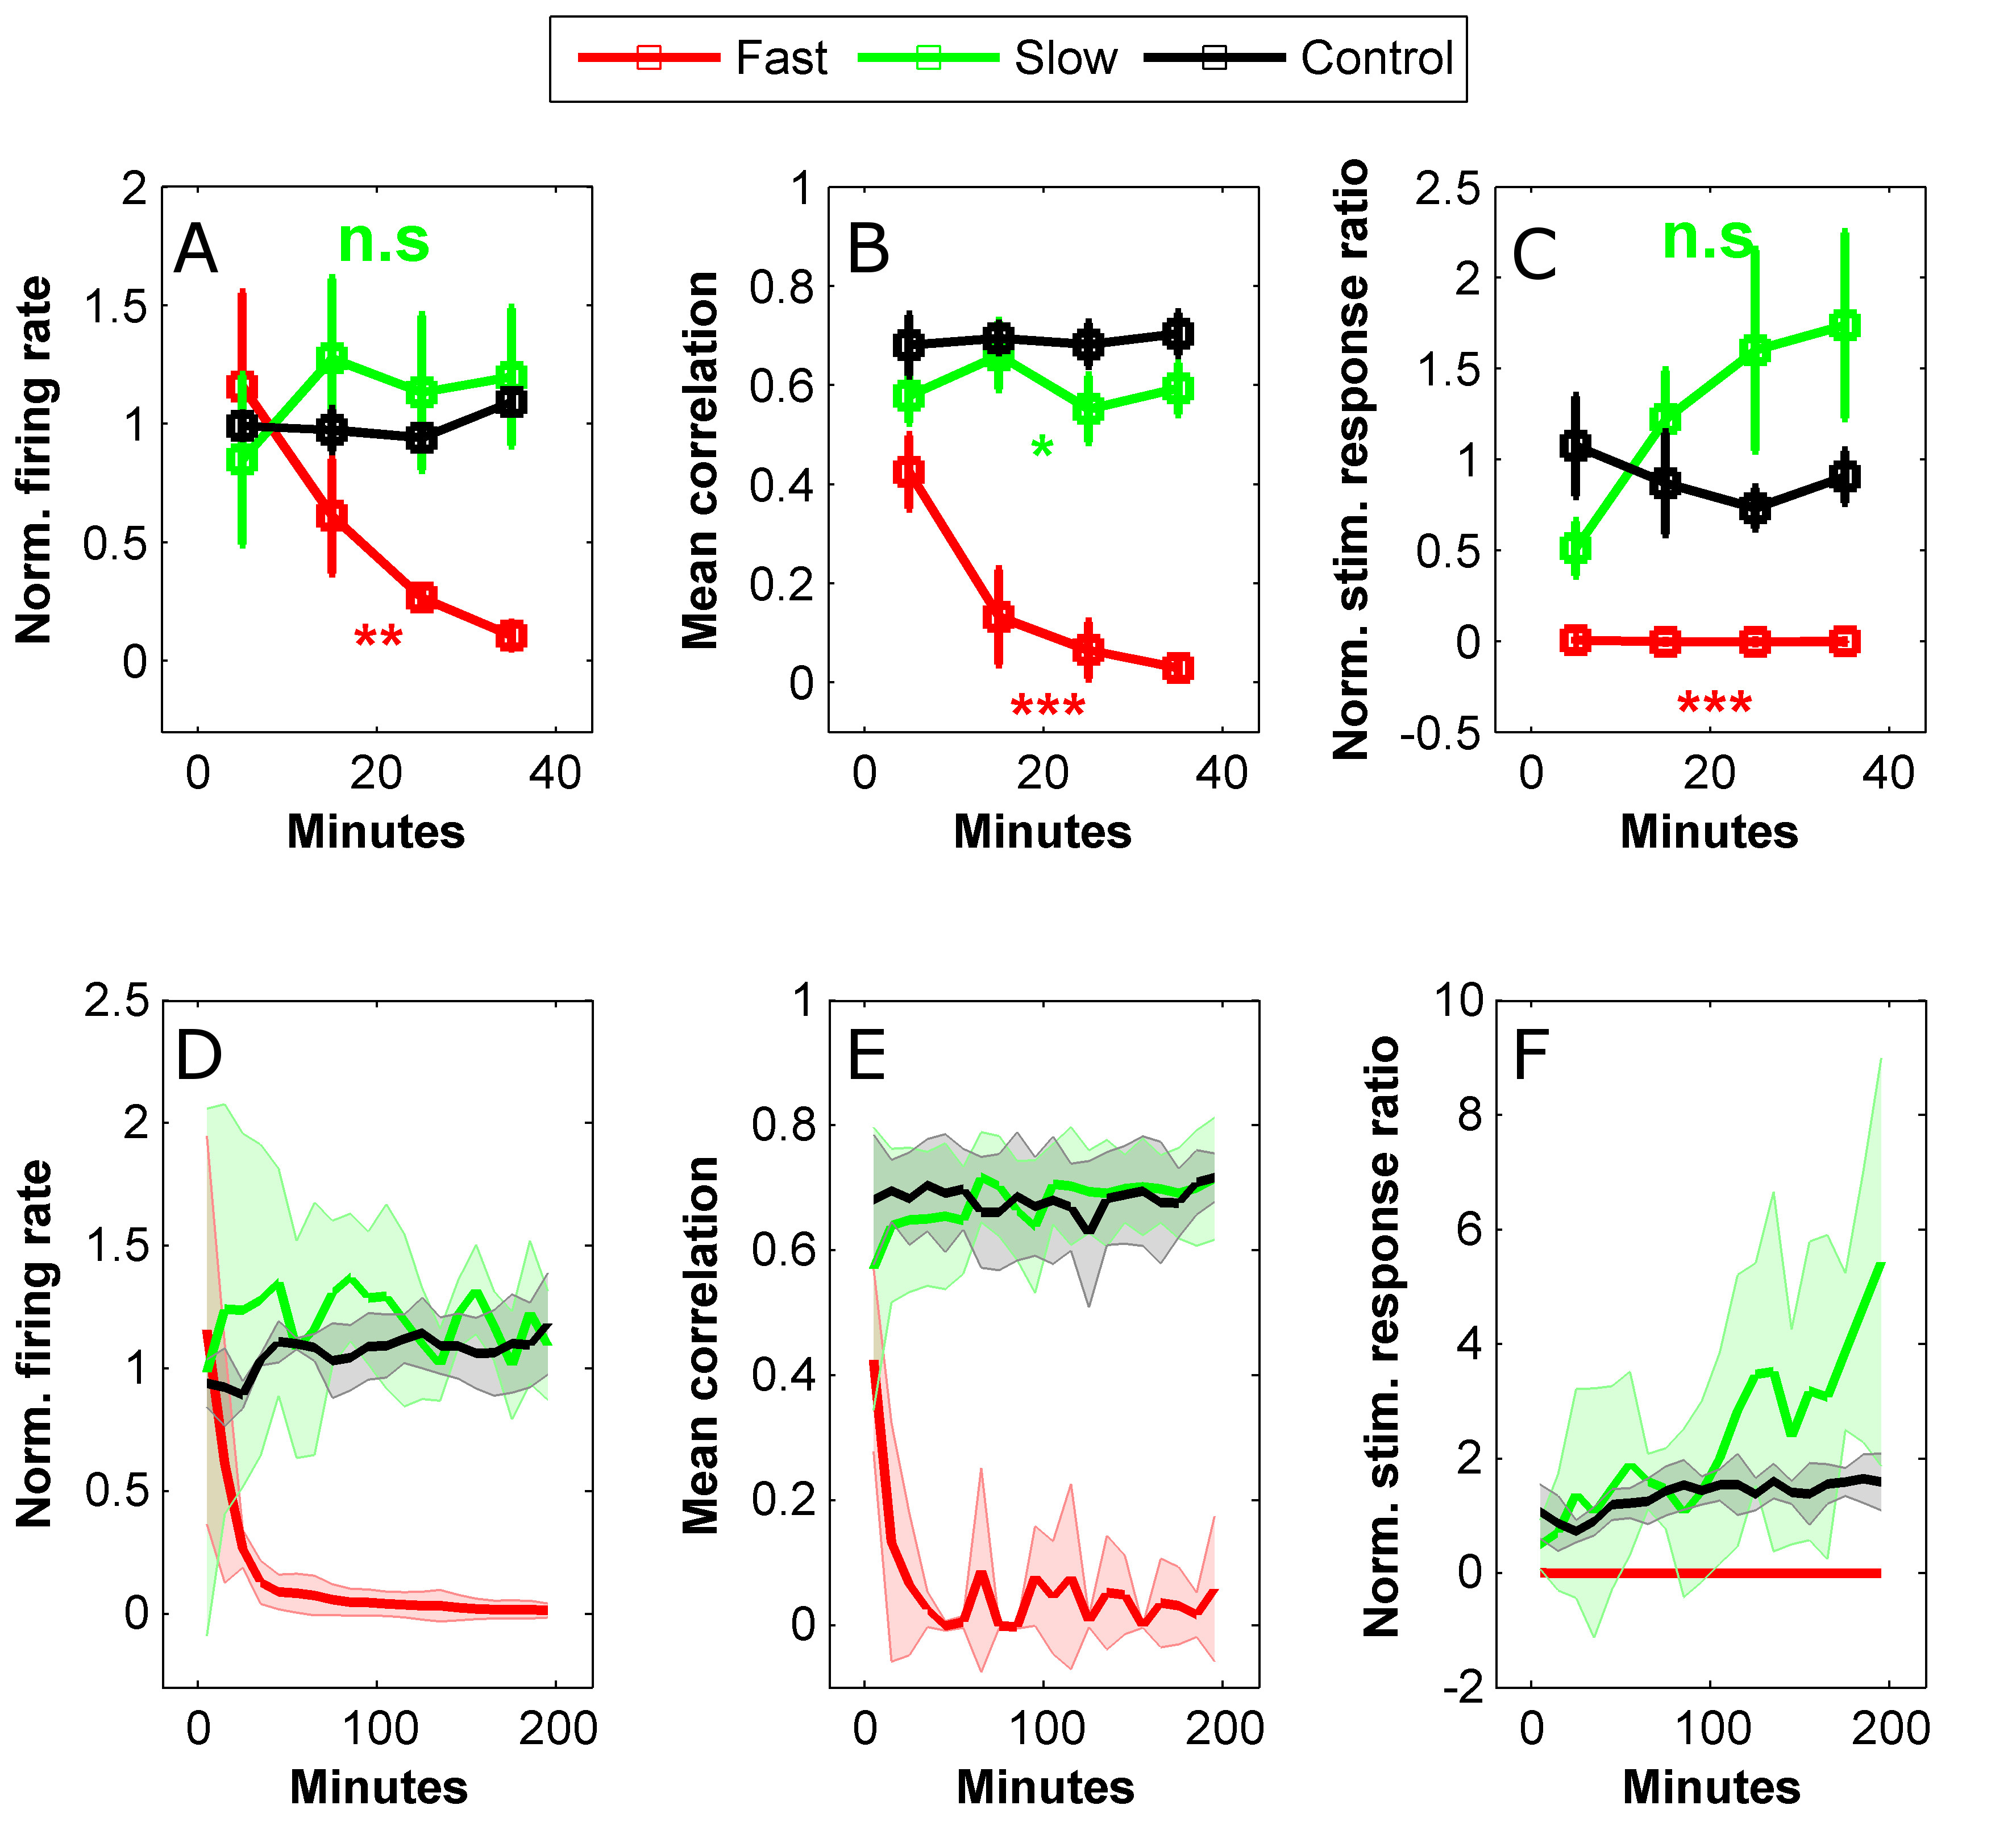
\includegraphics[width=15cm]{chapter5/figures/slowFastStats/slowFastStats.jpg}
            \caption[Averaged time course of activity measures in young cultures placed under flow at different rates]{\textbf{Young cultures placed under flow with self media suffer a flow rate dependent disruption to the activity which does not recover over time.} (A-C) Averaged measures of firing rate, mean correlation and stimulation response ratio in a 40 minute interval immediately after initiation of flow for 2 different flow rates and for recordings in static conditions (color coded). The measures are calculated in 10 minute bins. Error bars indicate SEM. A detailed definition of the measures can be found in the text. Time course of the 3 measures for the 2 flow rates is compared to control by means of a 2-way ANOVA. The statistical significance is determined by the lowest of the p values for group and interaction effects and is indicated by *, **, ***, n.s which refer to confidence levels of 95\%, 99\%, 99.9\% or \textless95\%, respectively. (E-F) Same measures as in A-C in an extended observation period of 200 minutes. All 3 measures crash immediately with fast, but not slow, flow onset. Shaded area represent the standard deviation of the measures. Firing rate and stimulation response ratio measures are normalized to their averaged value in the baseline recording prior to flow (or to the first hour in the case of the control). Data are based on n=4, 5 and 3 experiments for the fast flow, slow flow and control conditions, respectively.}
            \label{fig:crossFlow:slowFastStats}
        \end{figure}


        \subsection{The semi-permeable membrane approach for shear reduction}
        \label{sec:crossFlow:membrane}
        The results in the previous section reveal a flow rate threshold which cannot be exceeded if the culture is to maintain a stable network activity. Unfortunately, using direct flow at the permissive rate is incompatible with the rapid drug delivery which is the concern of this work and which requires flow speeds in the order of \(1 \frac{mm}{s}\) (see section \ref{sec:devices:protocolDev}). Thus we decided to explore an approach of decoupling the flow from the cells by means of a semi-permeable membrane. In this approach high flow rates would be maintained over the membrane to allow rapid drug delivery to the cell area above the membrane. The next step of the delivery would then be carried out via diffusion / slow convection through the membrane. Since the membrane can be positioned in close proximity to the cells the second delivery can potentially be made a quick as necessary. After all it is known that neurons use diffusion over short distances for inter-cell signalling which can be extremely fast (e.g., synapses). For example, if a \(10 \mu m\) membrane was to be positioned \(5 \mu m\) above the cells giving a total of \(15 \mu m\) drug travel distance then, by using the estimated diffusion time relation \(t\approx \frac{x^2}{4D}\) with \(D=400\frac{\mu m^2}{s}\) (typical diffusion coefficient value for a neurotransmitter sized molecule \cite{johnstoneThesis}), the drug delivery time would be \(\approx 140 ms\) which is easily compatible with the total required drug pulse time scales. In the case of the devices used here the height of the cell compartment is dictated by the thickness of the tape \(\approx 100\mu m\) so the distance is far greater than that required for rapid delivery. However, the aim here is to test the applicability of the approach and the correct distances can be implemented as needed in drug pulsing devices. Indeed this approach has been implemented before for shear free agonist gradient generation to cultured neurons \cite{morel2012amplification,morel2012concentration}. In that study an analytical estimate was developed for the maximal flow speeds which could be experienced by the cells underneath the membrane as a function of the flow speed over the membrane, of the membrane properties and of the device geometry. Applying this estimate to our devices provides a flow speed of \(20 \frac{nm}{s}\) in the cell compartment at most for the highest possible flow speed over the membrane. This estimate is 2 orders of magnitude lower than even the slow flow rate that was shown to be permissive of proper electrophysiological function in section \ref{sec:crossFlow:slowFast} so this approach holds a potential to sustain the network function.

        \begin{figure}[!htb]
            \centering
            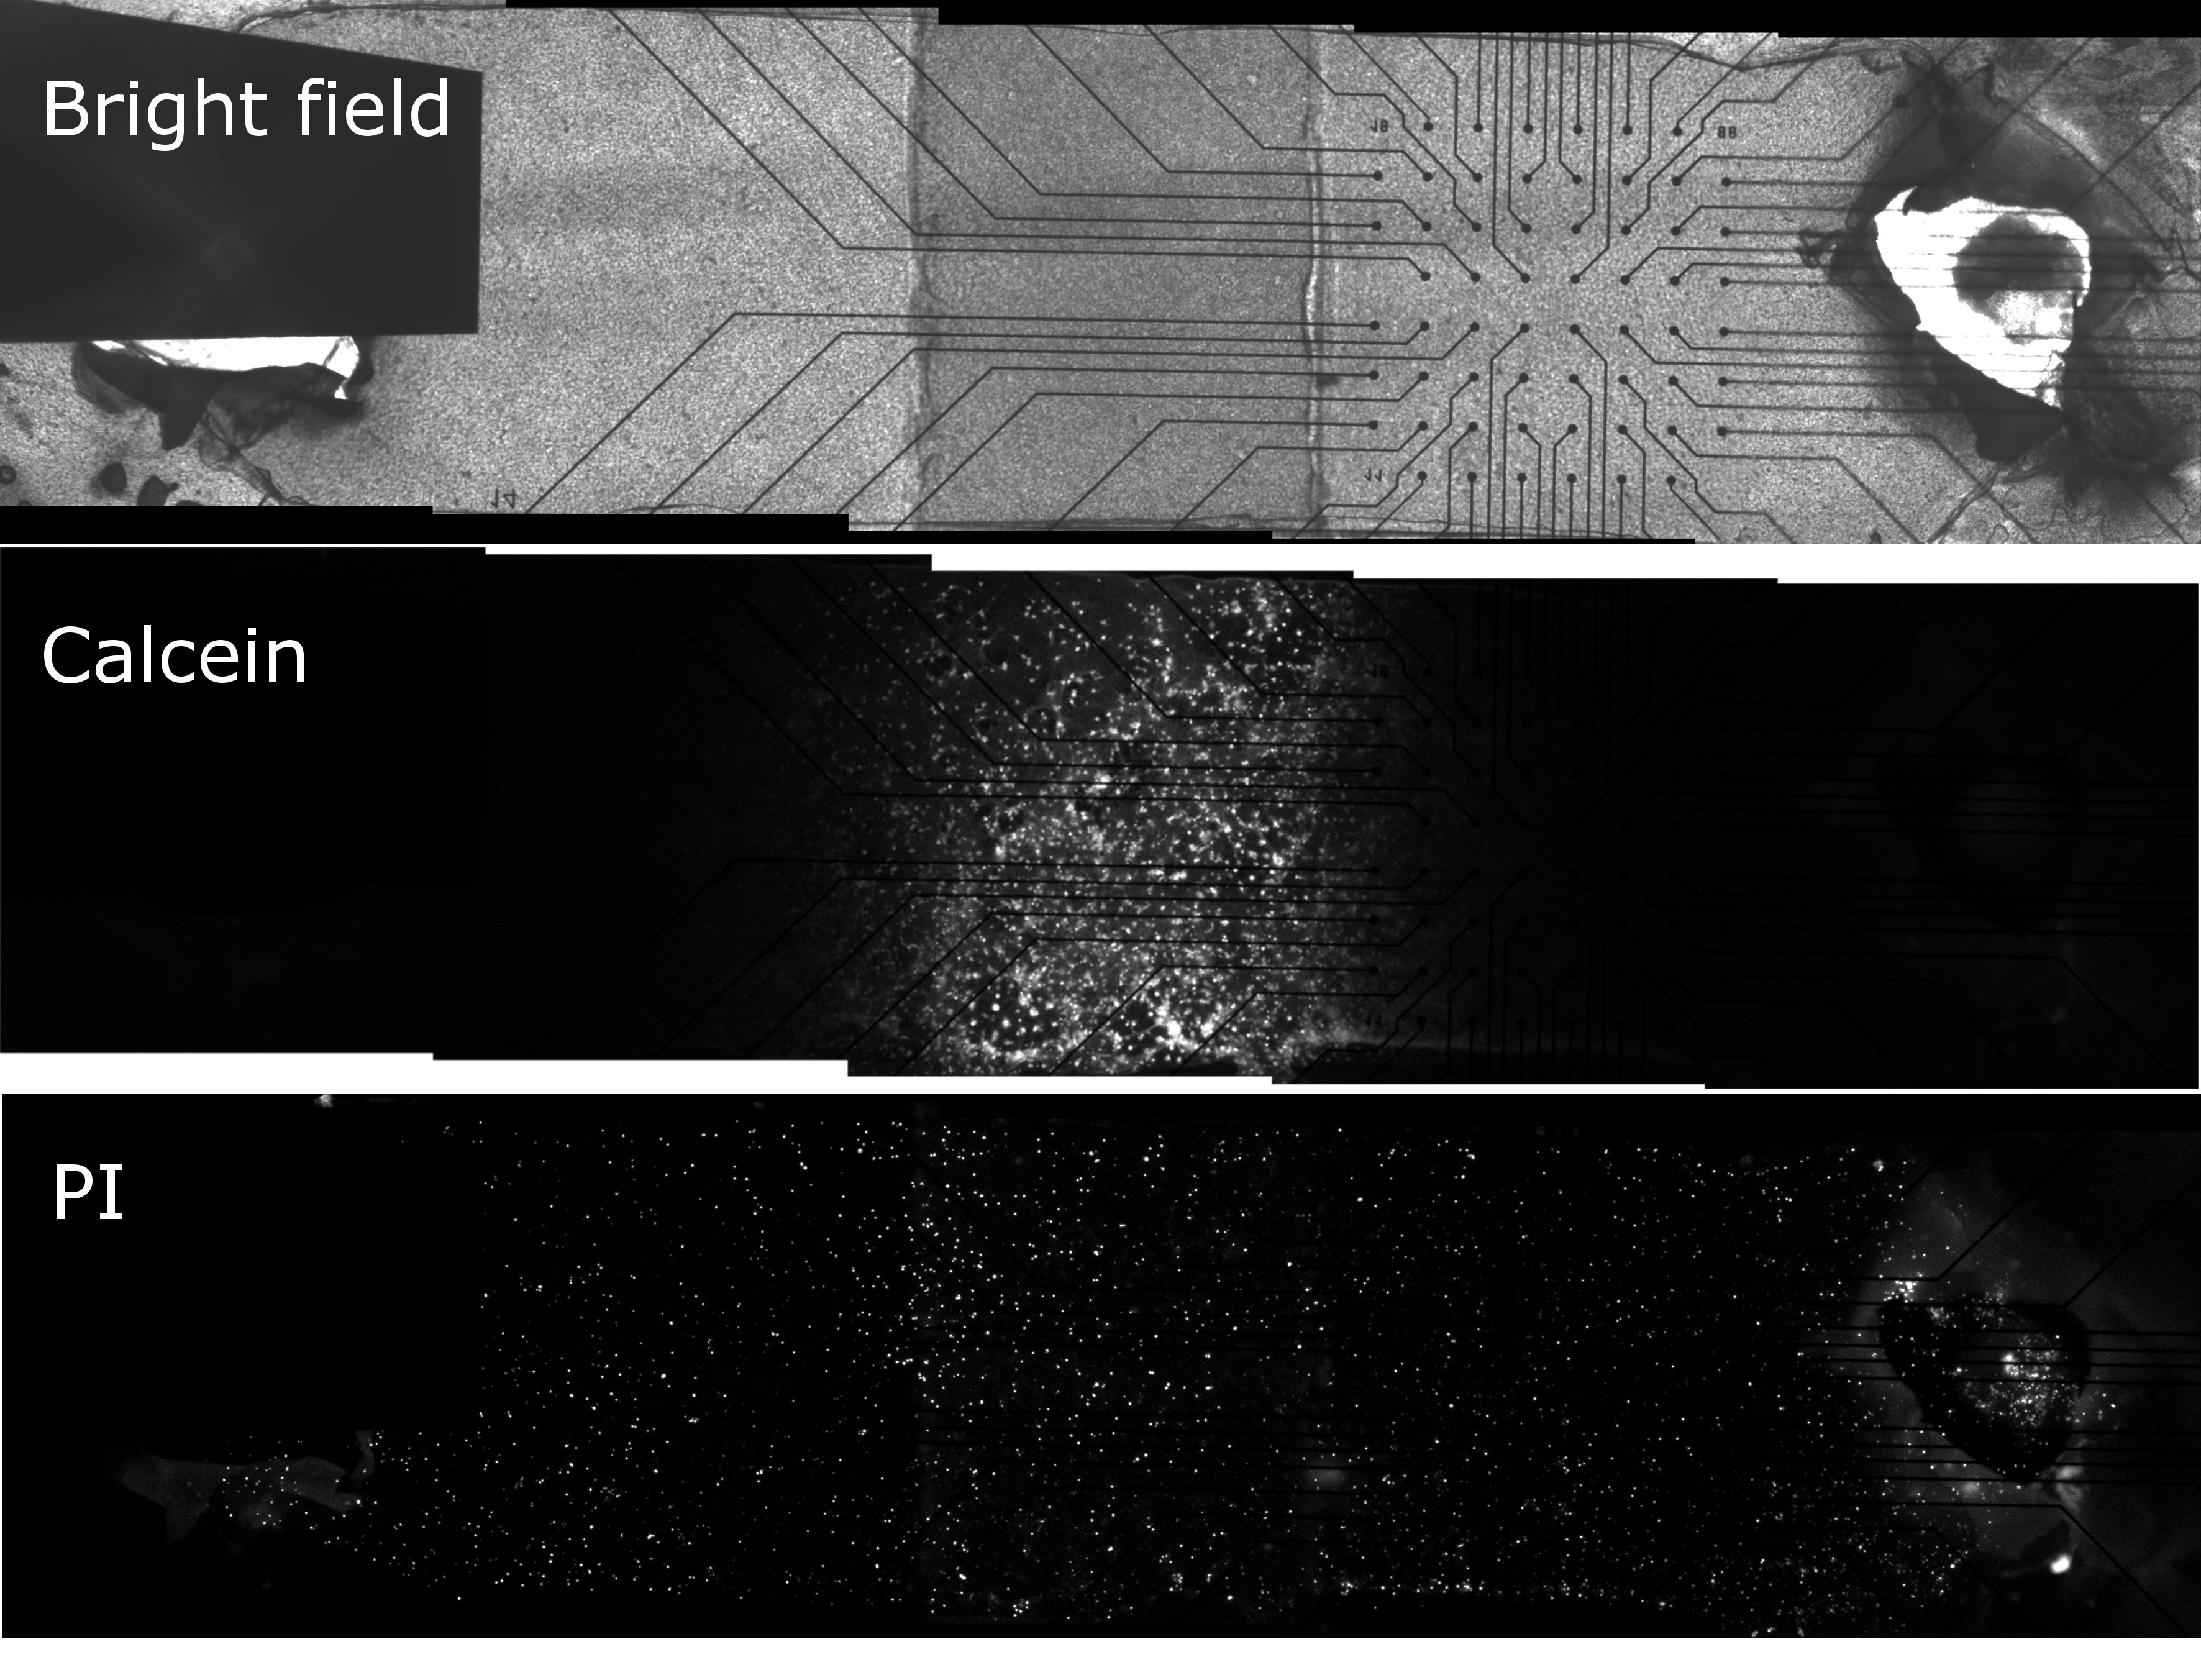
\includegraphics[width=15cm]{chapter5/figures/shiftedMembraneImage/shiftedMembrane.jpg}
            \caption[Bright field and staining images of a culture in a cross flow device inclusive of a semi-permeable membrane]{\textbf{Dead live stained Neuronal culture in a semi-permeable membrane device}. Polycarbonate membrane is not optically clear so cells are hard to distinguish in bright field image. The culture had been under flow with propidium iodide (dead cell stain, see sections \ref{sec:methods:flow} and \ref{sec:devices:viabilityAssay}) for 8 hours so the stain had diffused through the membrane opening to the extents of the culture channel. The live cell stain, Calcein-AM, had been introduced into the flow line only for the final 30 minutes of the flow session so that staining is present only immediately underneath the membrane opening. In this case the recording pads were not positioned directly under the membrane opening but rather shifted to one side.}
            \label{fig:crossFlow:shiftedMembrane}
        \end{figure}

        Young cultures growing in membrane devices were subjected fast flow under the same protocol as in the previous section (figure \ref{fig:crossFlow:shiftedMembrane} shows images of a culture stained following one such experiment). The results are compared to the fast flow on the non-membrane devices in figure \ref{fig:crossFlow:fastMembraneStats}. Remarkably, the introduction of the membrane did nothing to change the effect of the fast flow on the culture activity with all observed measures crashing with a very similar time course to that of the non membrane devices.

        We also include here the data from a single experiment where the MEA central area which contains the recording pads was not located directly underneath the membrane but was shifted to be entirely inside the non exposed area (figure \ref{fig:crossFlow:shiftedMembrane}). Since this was only a single experiment it cannot be included in a rigorous hypothesis testing analysis so it shown only in the long term plots for impression. This experiment did not include electrical stimulation. The recorded activity and the synchronicity in this case maintained a stable level for the full extent of the flow session. The level of synchronicity was markedly low compared to control but nevertheless stable. These data demonstrate that culture regions which are not placed directly underneath the membrane opening are able to maintain stable electrophysiological function. This experiment provides a positive control for the type of coupling that the culture can have with a flow environment while still sustaining its activity.

        \begin{figure}[!htb]
            \centering
            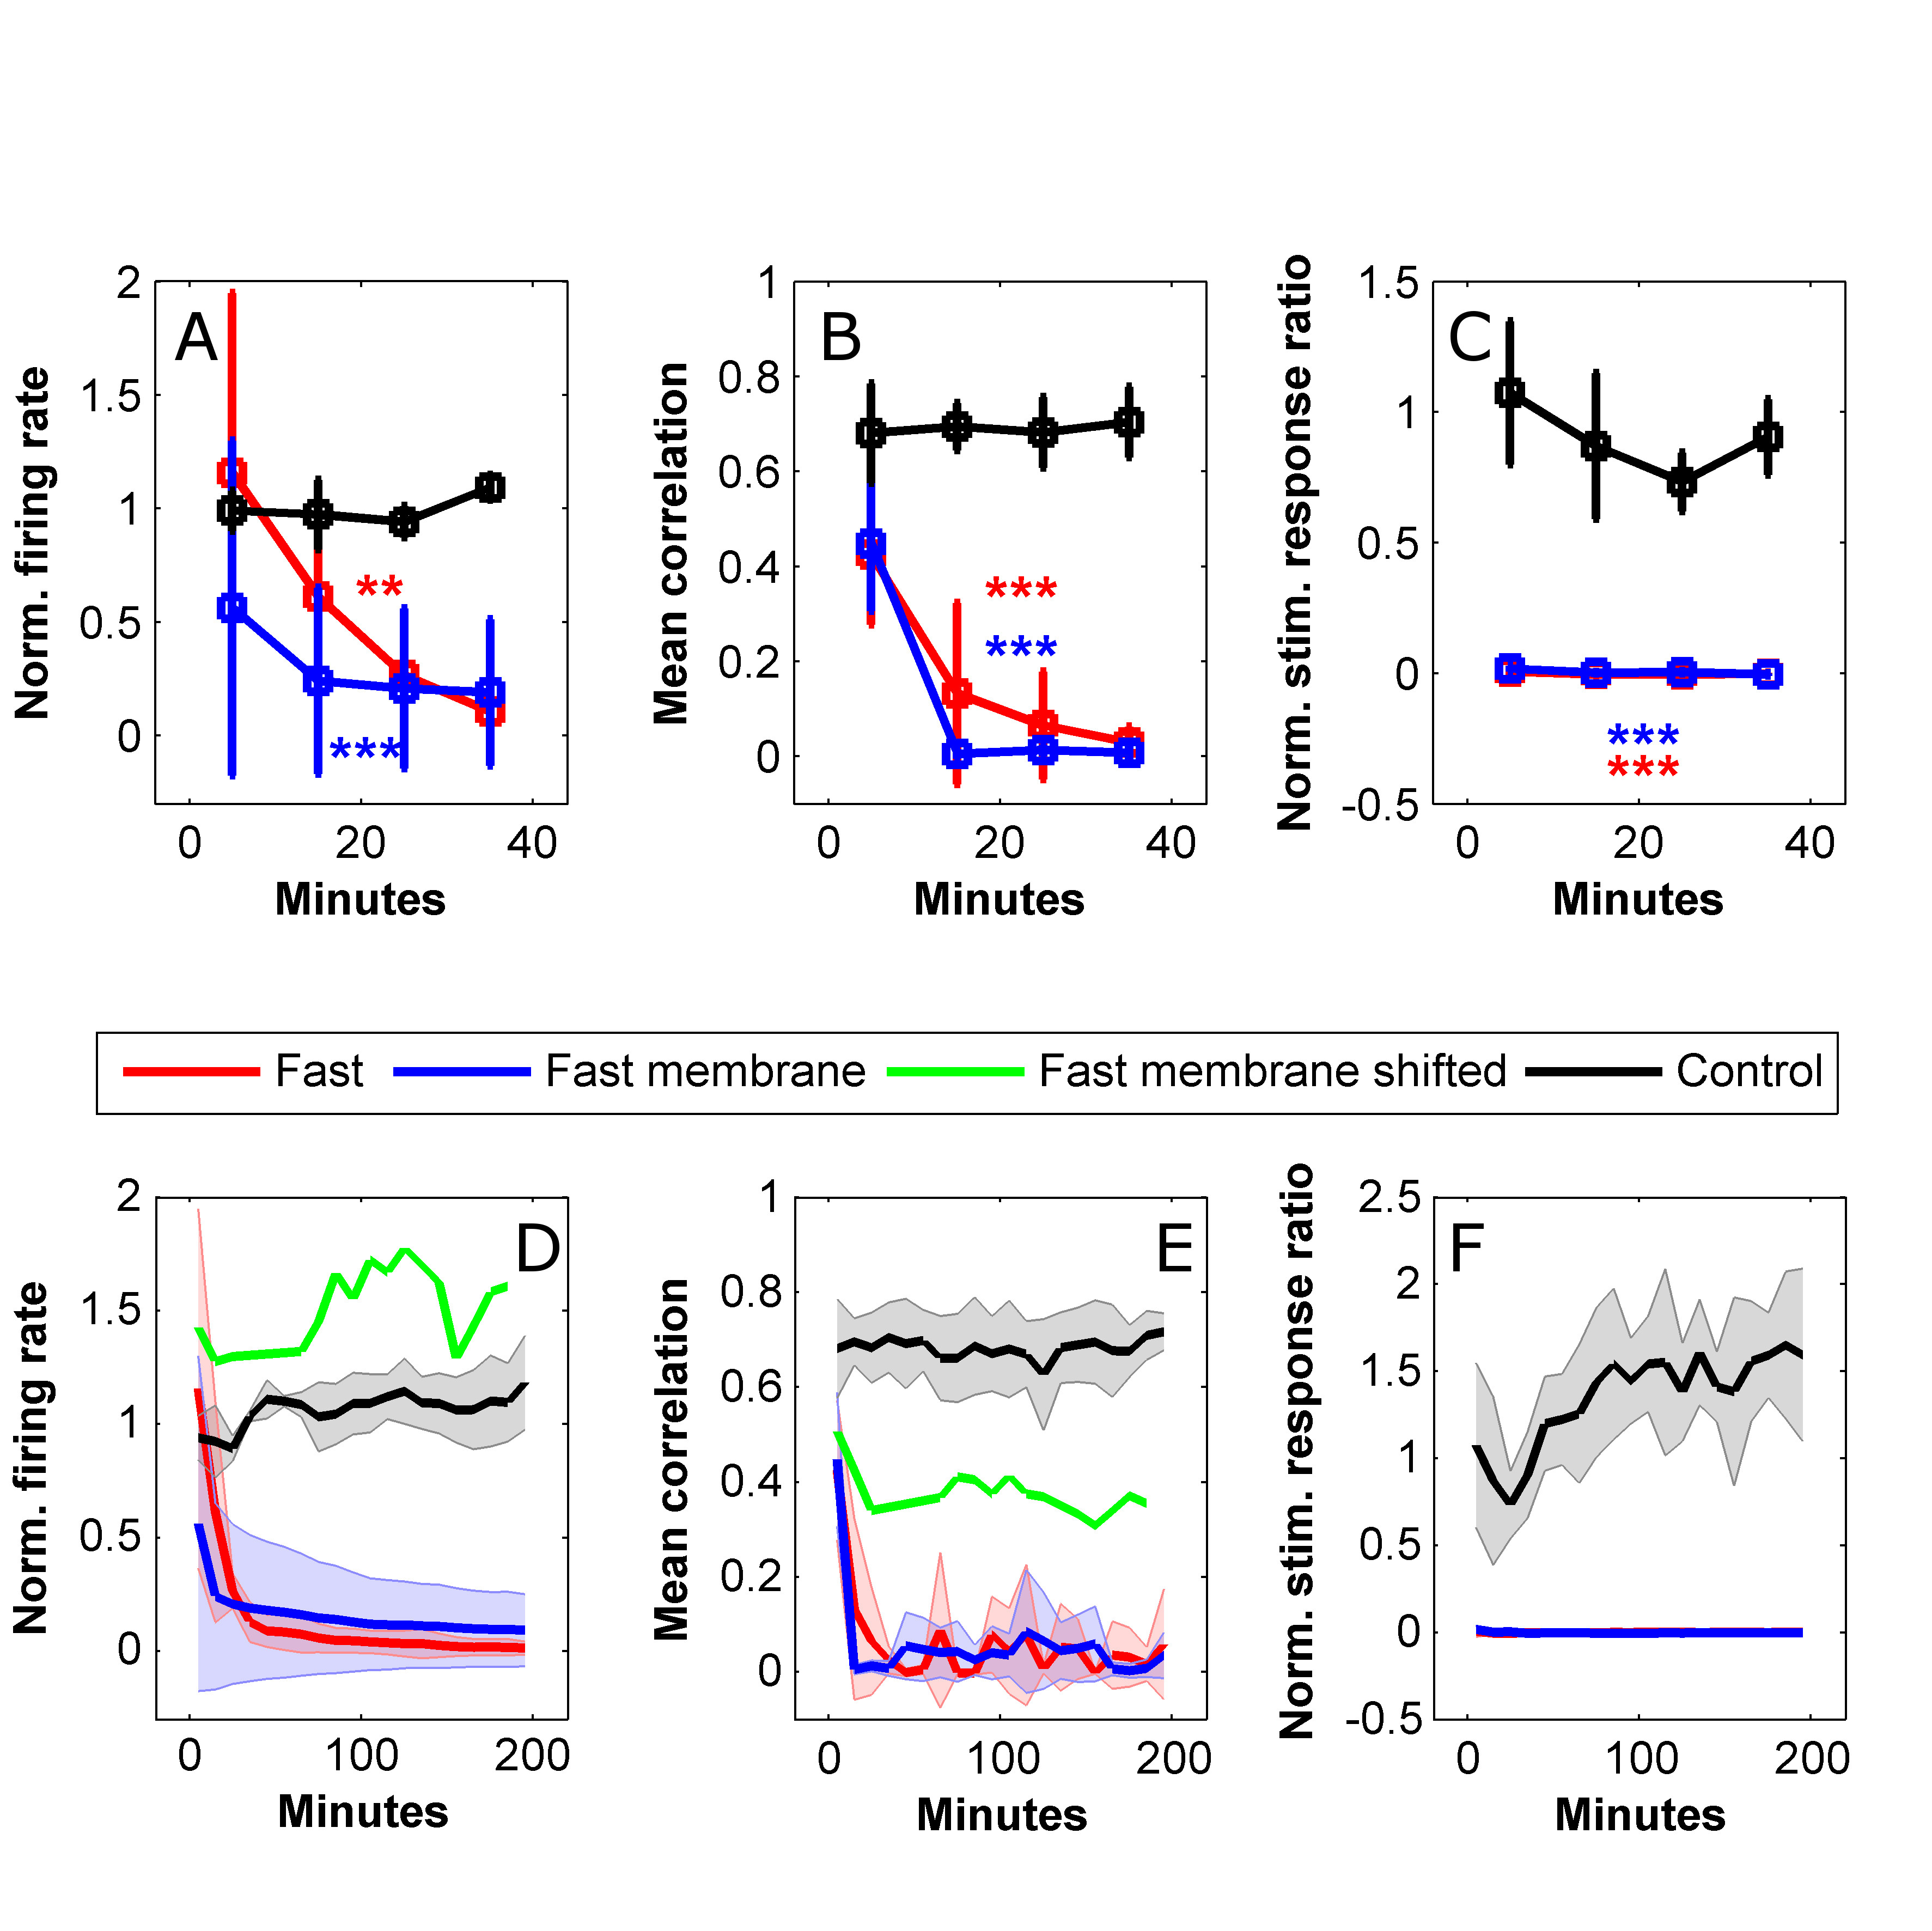
\includegraphics[width=15cm]{chapter5/figures/fastMembraneStats/fastMembraneStats.jpg}
            \caption[Averaged time course of activity measures in young cultures separated from the fast flow by means of a semi-permeable membrane]{\textbf{Introduction of a semi permeable membrane to decouple the cells from the flow does not improve the activity disruption under fast flow.} Measures are as in figure \ref{fig:crossFlow:slowFastStats} which also contains further information about the data presentation. Note the flow over the membrane (i.e., with \(\approx 100\mu m\) distance imposed between the flow interface and the culture) generates exactly the same effect as direct flow. Data are based on n=4, 3, 3, 1 experiments for conditions of fast flow, fast flow with membrane, control and membrane with shifted recording, respectively.}
            \label{fig:crossFlow:fastMembraneStats}
        \end{figure}

        \subsection{Considerations of diffusive flux}
        The above showed that despite the presence of the membrane the disturbance to the network activity remained as it was before. At first glance, this is surprising because one would expect that the decrease in convective flux due to the presence of the membrane would assist in both in diminishing the shear stress and in maintaining a stable chemical environment under the membrane. Thus it could be expected that regardless of the cause of the disturbance, shear stress or convective flux, the membrane should afford protection. However, this intuition does not take into account the diffusive flux which becomes dominant for short distances. Thus, in what follows, we compare the diffusive flux present in the case of the membrane experiments to the convective flux induced by the slow flow.

        Considering a certain conditioning factor species which is produced by the culture and normally present at a concentration \(C \frac{moles}{\mu L}\). Then in the case of direct flow through the channel this species would be carried away by the flow and removed at a flux:

        \[J_{conv}=QC=1\times 10^{-3}C \frac{moles}{s},\] where \(Q=1\times 10^{-3}\frac{\mu L}{s}\) is the volumetric flow rate for the slow flow.

        In the case of the membrane experiments, we assume that the aforementioned conditioning species is not present in the flow media so its concentration over the membrane is null. We further assume a linear concentration gradient for the species between the cells and the top of the membrane. Then, according to Fick's law the diffusive flux density between the membrane from the cells across the gap and through the membrane is: \[j_{diff}=D\cdot\frac{C}{h}=4\times 10^{-3}C \frac{moles}{s\cdot mm^{2}},\] where \(D=4\times 10^{-4}\frac{mm^2}{s}\) is the diffusion coefficient for neurotransmitter sized molecules and \(h=0.1 mm\) is the height of the cell compartments. To get the total flux through the membrane we multiply the flux density by the area of the membrane opening \(A=4 mm^{2}\): \[J_{diff}=j_{diff}\cdot A=1.6\times 10^{-2}C\frac{moles}{s}.\] Thus the total diffusive flux of the considered conditioning species through the membrane is actually more than an order of magnitude \textbf{higher} than its convective flux during the slow flow experiments. It should be noted that the above calculations include only diffusive flux for the membrane scenario and therefore subliminally assume that the membrane is an ideal diffusive barrier. However, in the case of a real membrane (which is never ideal) the removal flux would be yet more extreme. Another heuristic which emerges from these calculations is that the diffusive flux is inversely proportional to the height of the cell compartment (i.e., the distance between the neurons and chemical sink). In order to equalize the factor removal flux to that of slow flow scenario the membrane needs to be located about \(1-1.5 mm\) away from the cells. This would explain why standard perfusion systems, which exchange media only from the top surface of the culture bath do not exhibit issues with the network activity as seen here. This heuristic fits well with the results from the experiment where the recorded portion of the culture was shifted relative to the membrane opening. In that experiment the recorded cells were positioned at distances between \(400-2000\mu m\) from the membrane which means they were only partially in the `safe' region. Indeed the stable synchronized network activity in that experiment persisted but the effect of the flow was still evident through a decrease in synchronization level compared to the control.

        The diffusive flux considerations discussed here give rise to an important heuristic: drug delivery through a diffusive barrier designed to introduce a certain agonist at a given rate would inevitably remove agonists of a similar size at the same rate unless they are also present in the delivery media. The results of the membrane experiments, therefore strongly suggest that the self media used for flow does not fully reflect the chemical environment in the internal volume of the devices, even though it was extracted from the same culture dish. In the next section we provide evidence that, in the case of older cultures, this discrepancy is reduced thus providing means to achieve stable activity under rapid flow.

\section{Activity under flow for old cultures}
\label{sec:crossFlow:oldSelf}
        In this section we describe a set of experiments measuring the activity of cultures aged 20-23 days \textit{in vitro} placed under fast flow with various media formulations. Section \ref{sec:crossFlow:slowFast} described how, when young cultures were placed under fast flow with self media, the network activity was immediately abolished. Remarkably, when an identical experiment was performed on old cultures, the synchronized network dynamics persisted under flow with little interruption, namely with the spontaneous activity proceeding in the form of synchronized bursts, with high values in the correlation matrix and with stable responses to stimulation (figure \ref{fig:crossFlow:youngOldExampleRaster}). Nevertheless, the initiation of flow was still evident in some subtle yet distinctive changes to the activity structure. Specifically, some of the channels exhibited tonic discharges in discord with the bursts. This can be seen directly in the raster plots (figure \ref{fig:crossFlow:youngOldExampleRaster} A, right panel) and also in the correlation matrices which, despite generally maintaining their structure, contained some channels whose correlation values were reduced under flow (figure \ref{fig:crossFlow:youngOldExampleRaster} C, compare middle and right panels). Additionally, the stimulation responses intensified and became somewhat longer (figure \ref{fig:crossFlow:youngOldExampleRaster} B, right panel).

        \begin{figure}[!htb]
            \centering
            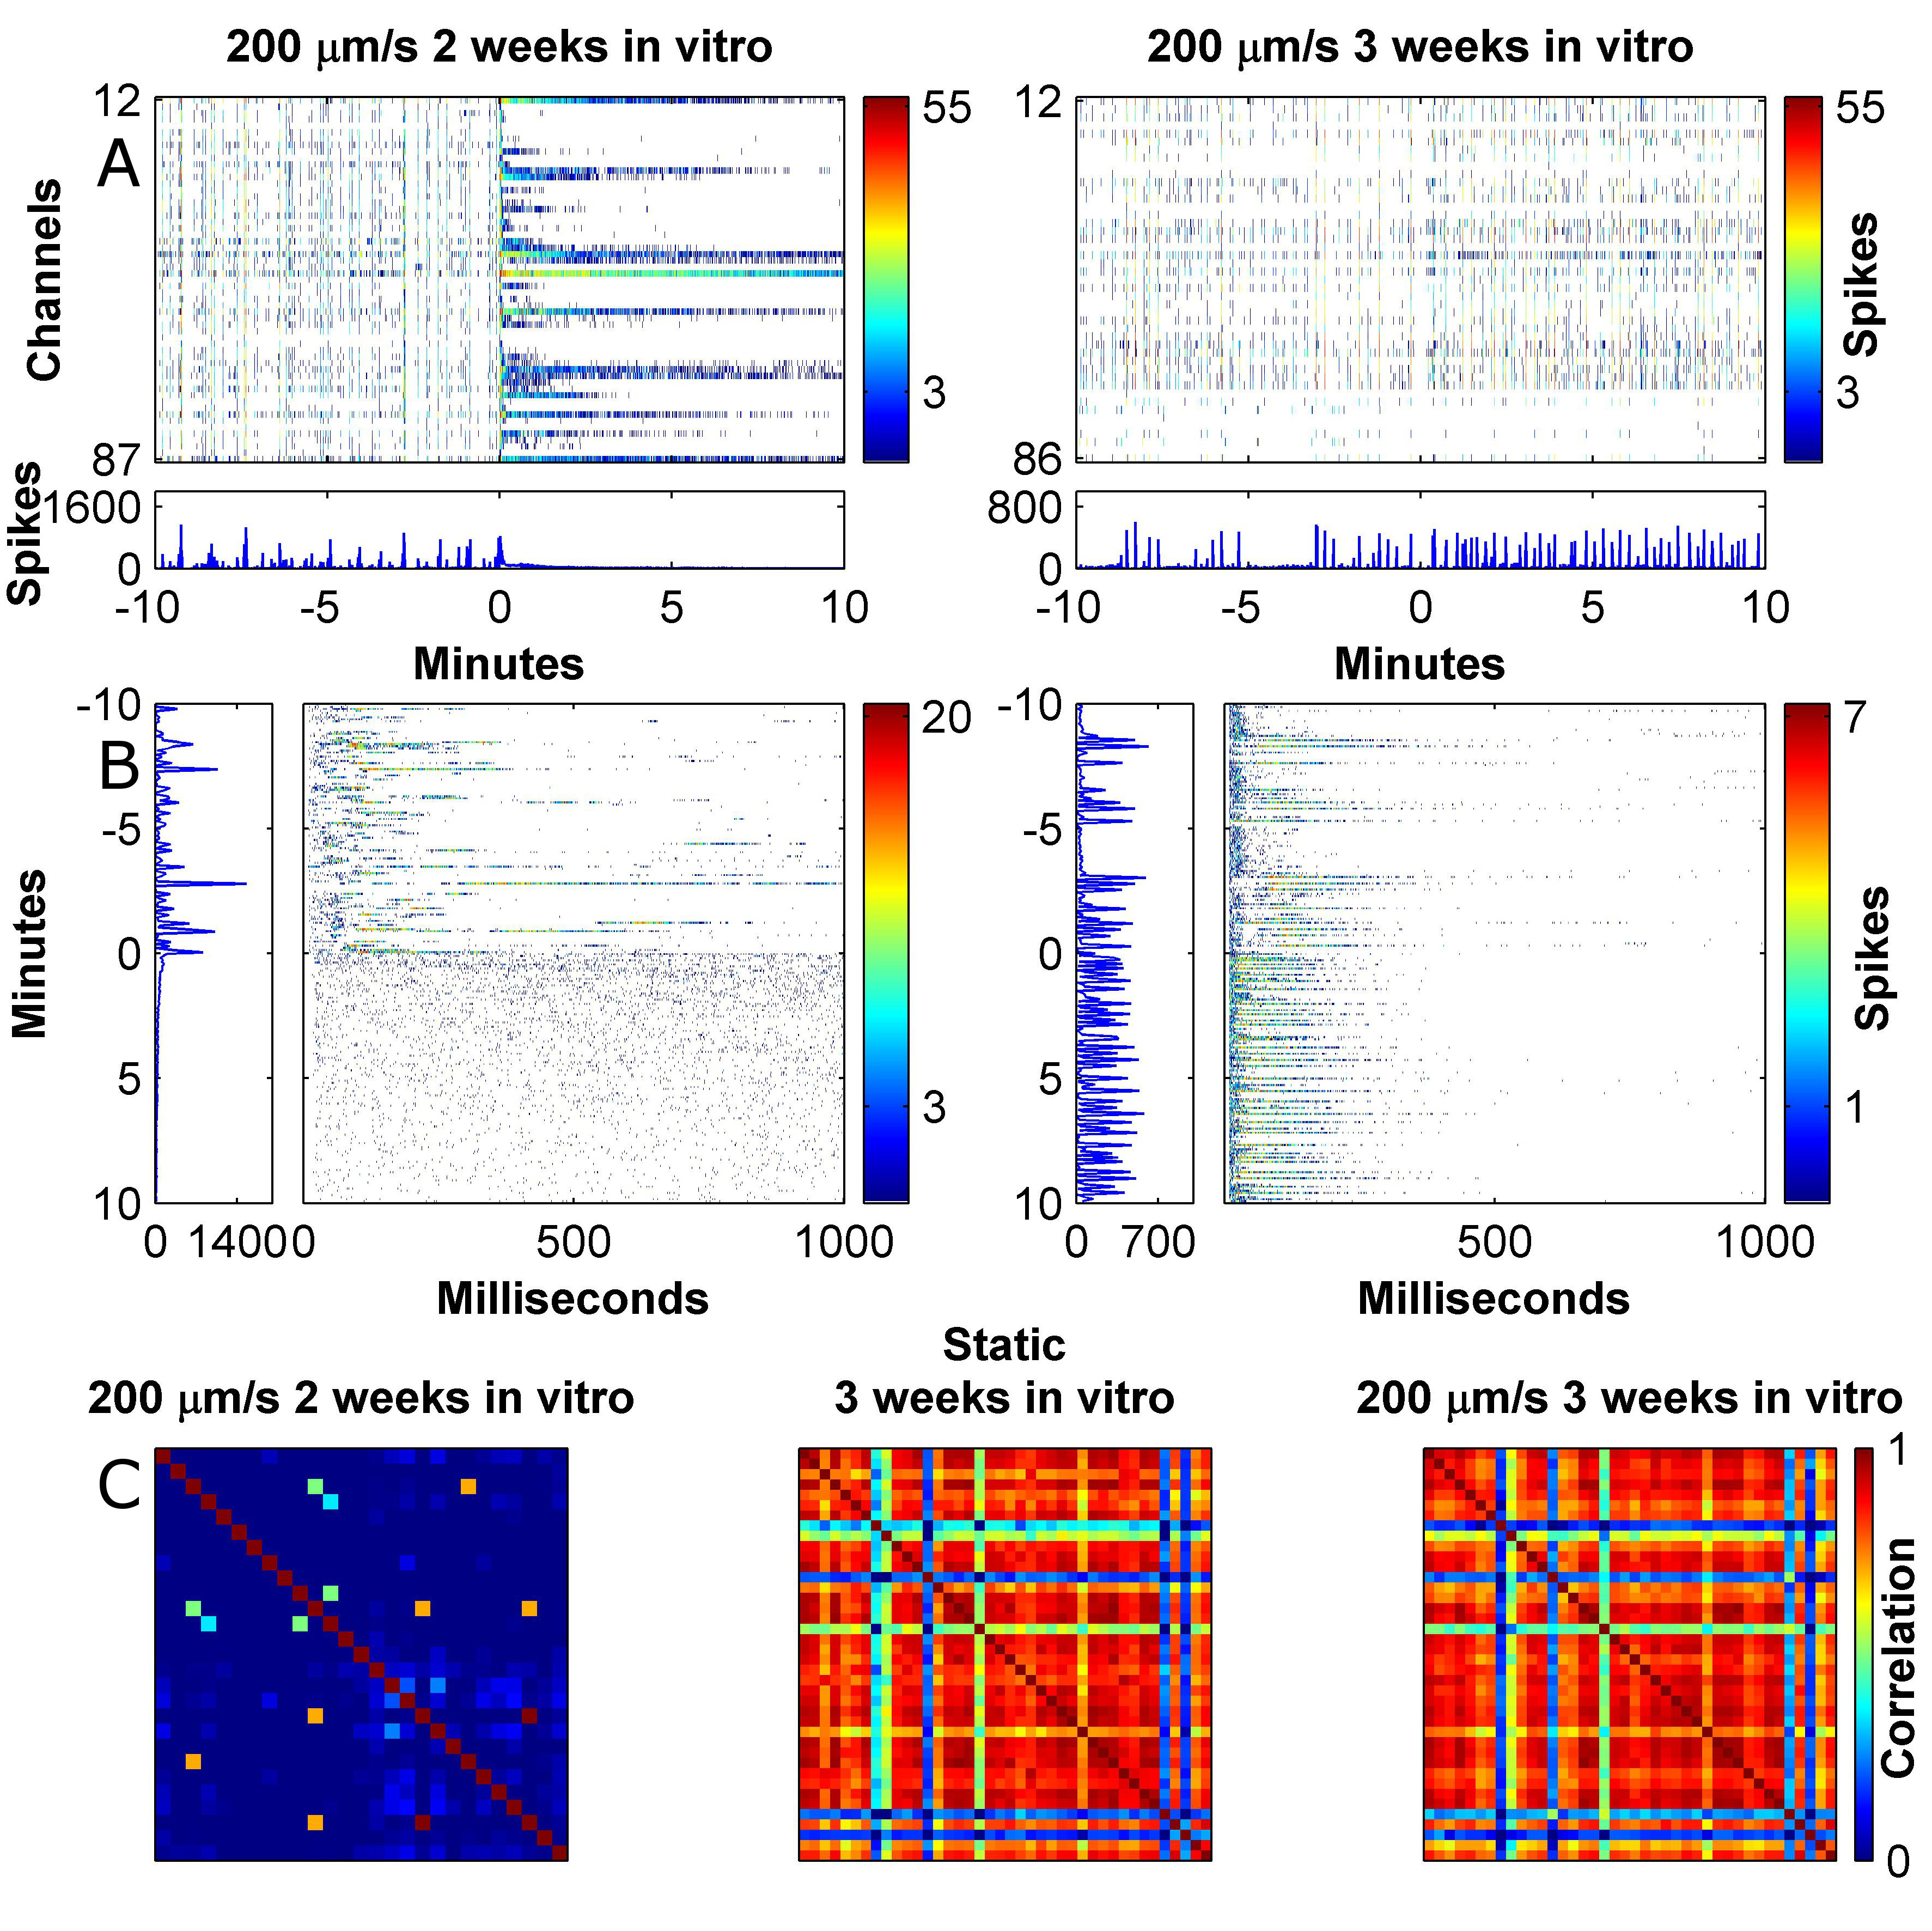
\includegraphics[width=15cm]{chapter5/figures/youngOldExample/youngOldRasterExample.jpg}
            \caption[Example for the effect of culture age on the network activity under flow]{\textbf{Old cultures under fast flow maintain a stable network activity.} Data presented as in figure \ref{fig:crossFlow:slowFastExample} only in this case two different cultures (young and old) are compared rather than flow rates on the same culture. In this case the activity and stimulation responses are maintained under fast flow with only small modulations. The correlation matrix for static conditions shows the data from the old culture before it was subjected to flow.}
            \label{fig:crossFlow:youngOldExampleRaster}
        \end{figure}

        The stability of activity under flow was consistent over several old cultures from several platings as is shown in figure \ref{fig:crossFlow:youngOldStats} which compares the 3 activity measures introduced in the previous section for  young and old cultures under flow as well as for control (static) cultures of the same age groups. The firing rate and synchronicity measures for old cultures are indistinguishable from their controls (2-way ANOVA, \(p=0.084\) and \(0.35\), respectively. P-values given are the minimum between the group and interaction effects). The reported lengthening of the stimulation response was manifested as a significant two-fold increase in the stimulation response ratio as compared to controls (2-way ANOVA, \(p=2.7\times 10^{-5}\)) but the response was stable throughout the observation period.

        \begin{figure}[!htb]
            \centering
            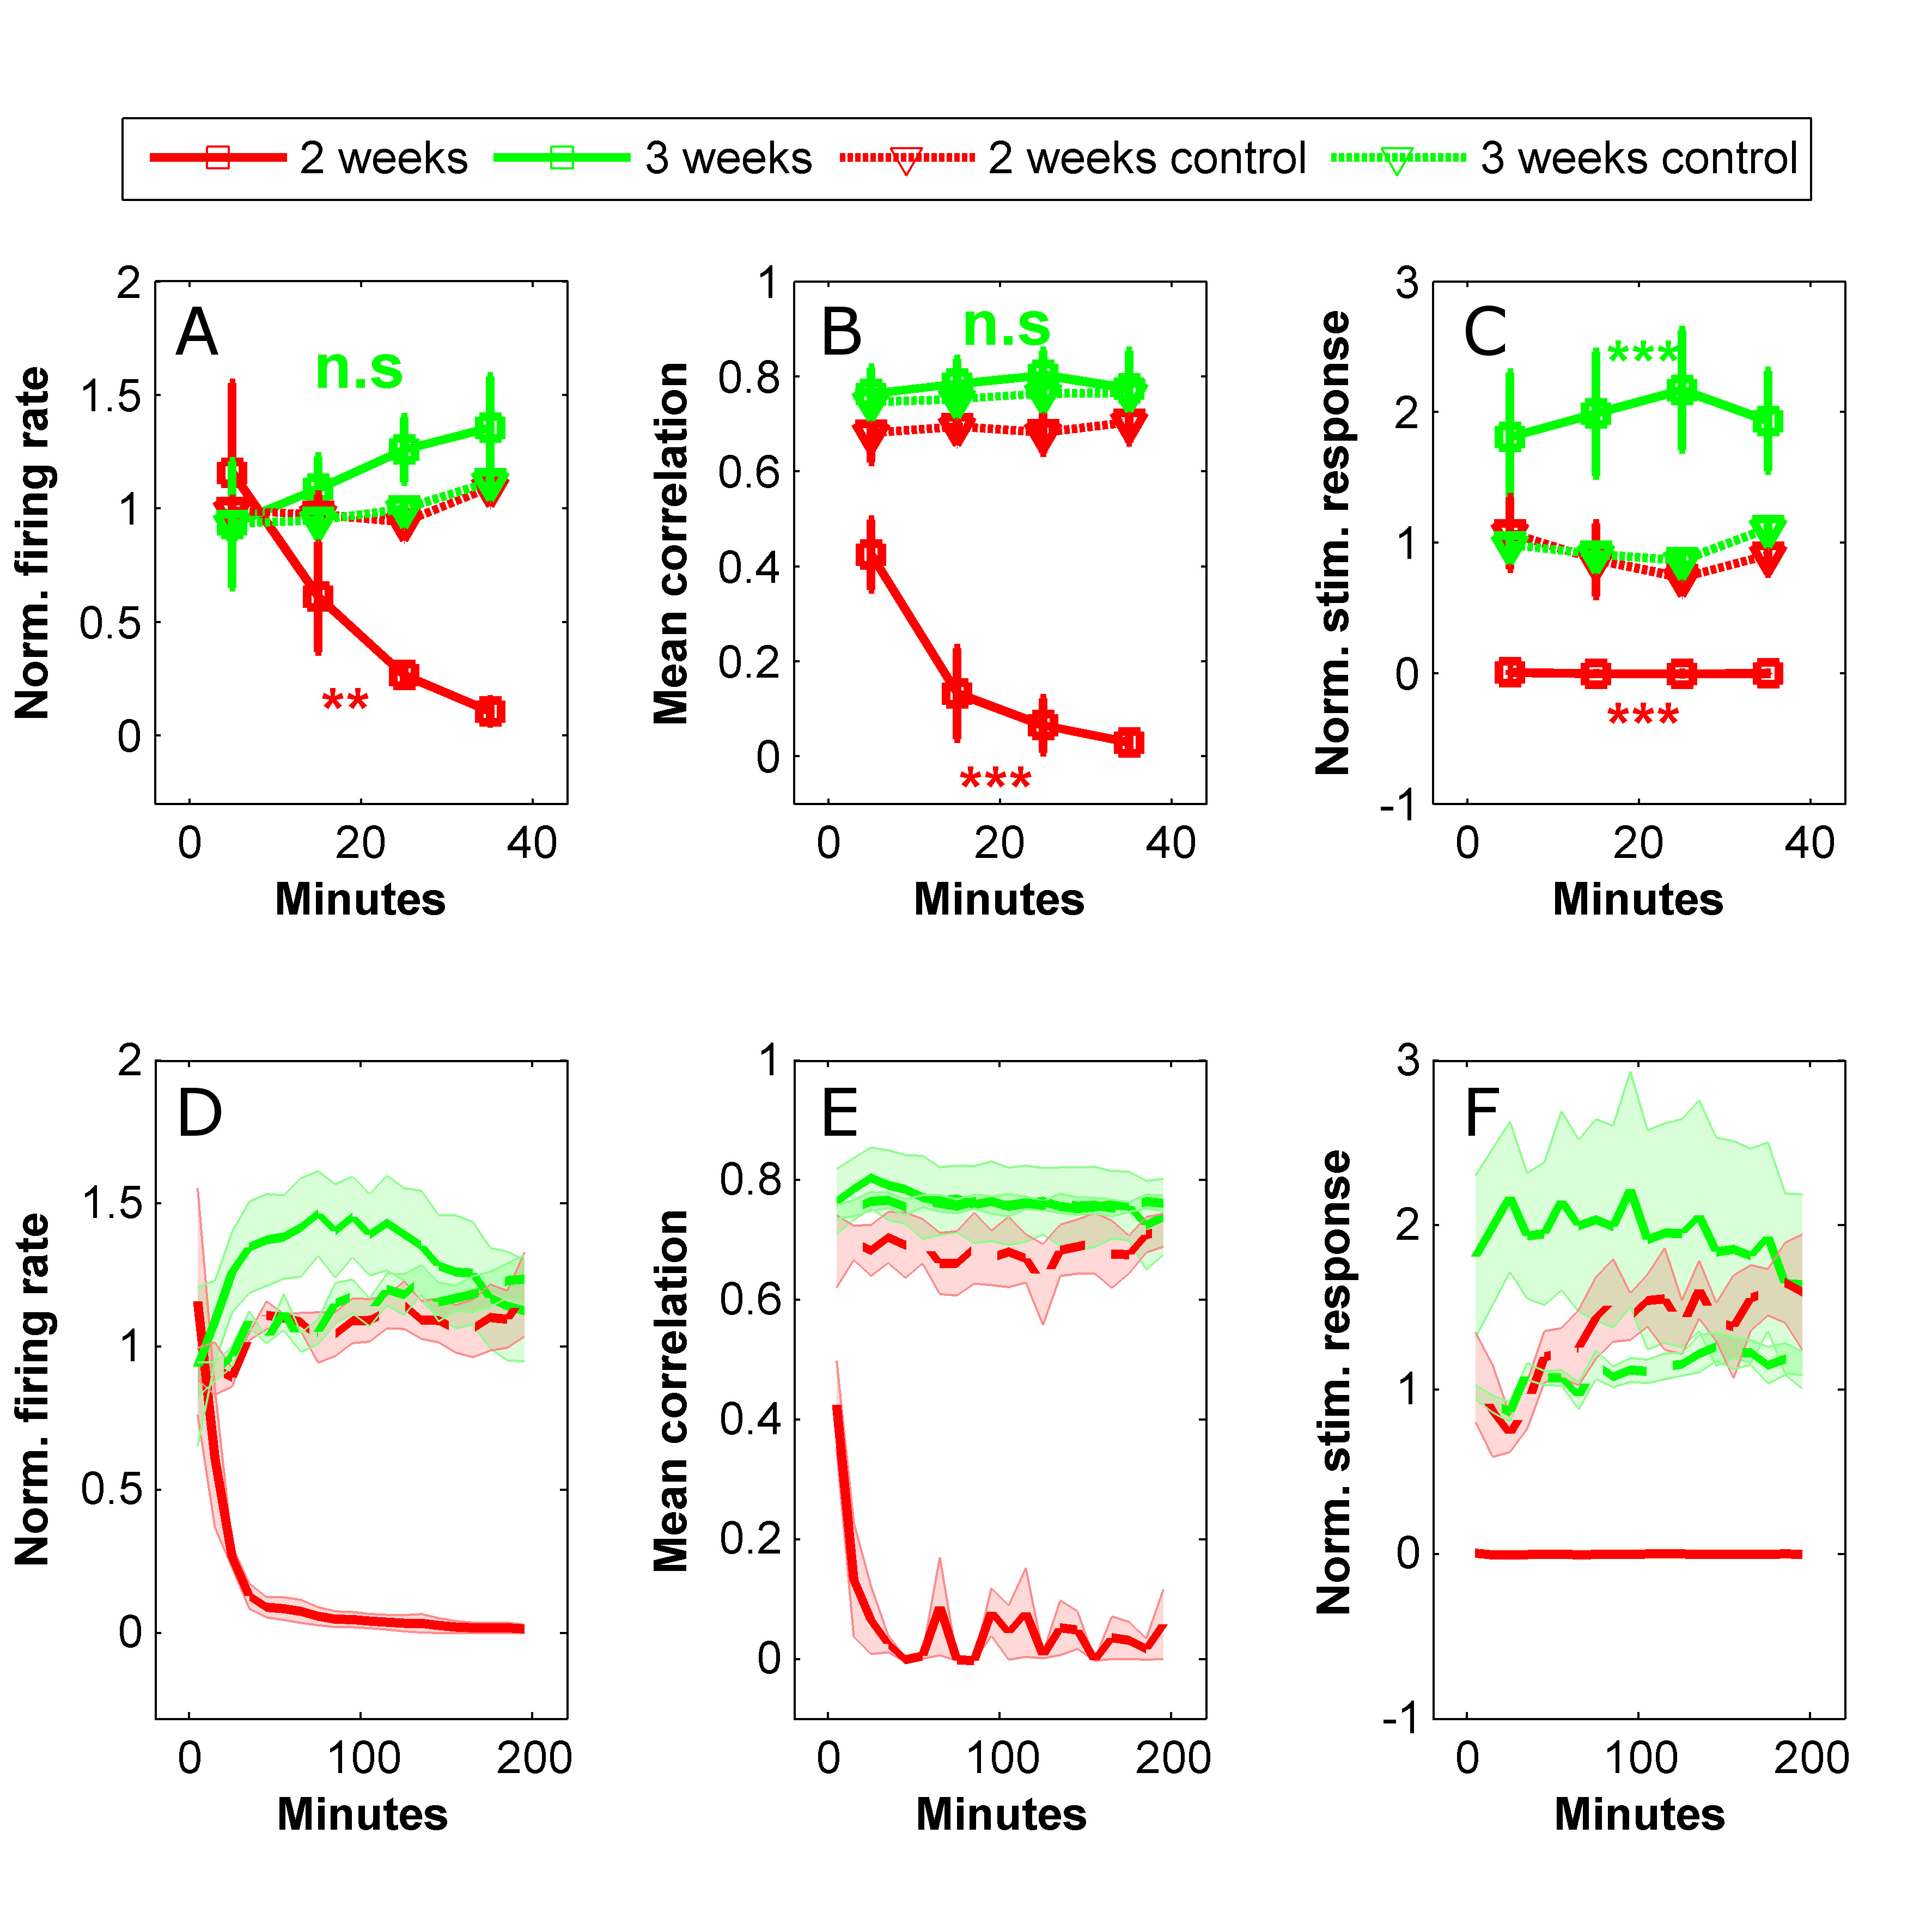
\includegraphics[width=15cm]{chapter5/figures/youngOldStats/youngOldGraphs.jpg}
            \caption[Averaged time course of activity measures in young versus old cultures under flow]{\textbf{Old cultures under fast flow maintain a stable network activity for and extended period of time.} Measures are as in figure \ref{fig:crossFlow:slowFastStats} which also contains further information about the data presentation. Data are based on n=4, 4, 3, 5 experiments for conditions of fast flow young, fast flow old, young control and old control, respectively.}
            \label{fig:crossFlow:youngOldStats}
        \end{figure}

        \subsection{The effect of the media source}
        It is quite evident from figure \ref{fig:crossFlow:youngOldExampleRaster} that young and old cultures are conspicuously different in their response to stimulation. In both cases the responses are bi-modal in strength, i.e., usually take the form of a short network reverberation of \(\approx 200 ms\) but occasionally produce a long response of a second or more. However, in the case of old cultures the short reverberations are stronger and more consistent as compared to young ones. As mentioned is section \ref{sec:activity:activityStats}, although synapse density peaks at the end of the 2\textsuperscript{nd} week \textit{in vitro} \cite{li2003some}, there is evidence that other synapse related processes such as pruning and changes to the GABA system still significantly affect the network dynamics at later stages (3\textsuperscript{rd} and 4\textsuperscript{th} weeks). The observed increase in the reliability of reverberative response to stimulation might be another manifestation of these later maturation processes although their exact nature is not completely understood. In the present context, it is possible that these age-related changes to the network structure render it more robust to environmental perturbations and therefore could explain why activity is maintained under flow with only minor perturbations. Another age related process which may have to do with the results is ECM formation. It is known that the ECM content in neuronal culture increases over the the 3\textsuperscript{rd} and 4\textsuperscript{th} weeks and that its presence facilitates synaptic function by preventing spill over \cite{bikbaev2015brain}. It is possible  that increased ECM content in the old cultures serves as a protective barrier which allows them to sustain the network activity under flow. The results of the membrane experiments in section \ref{sec:crossFlow:membrane} suggested that the self media lacks important conditioning factors which consequently get removed by the flow causing the activity disruption. It therefore possible that the developed ECM help to sustain a localized chemical environment by tethering important conditioning factors even if they are not present in the flow media. It is also possible that the more developed synapse formation renders the activity more stable and makes the culture insensitive to perturbation in the environment chemistry. We wanted to test if indeed old cultures are characterized by a reduced sensitivity to the culture media as this information could inform future flow applications. We therefore conducted two more sets of flow experiments. In the first one we used media from young cultures for flow. In the second one we used self media again but performed the experiments 1-3 days following a media change whereby 25\% of the culture's media was replaced with fresh media (the previous self media experiments in section \ref{sec:crossFlow:oldSelf} were performed 6-9 days following a media change).

        \begin{figure}[!htb]
            \centering
            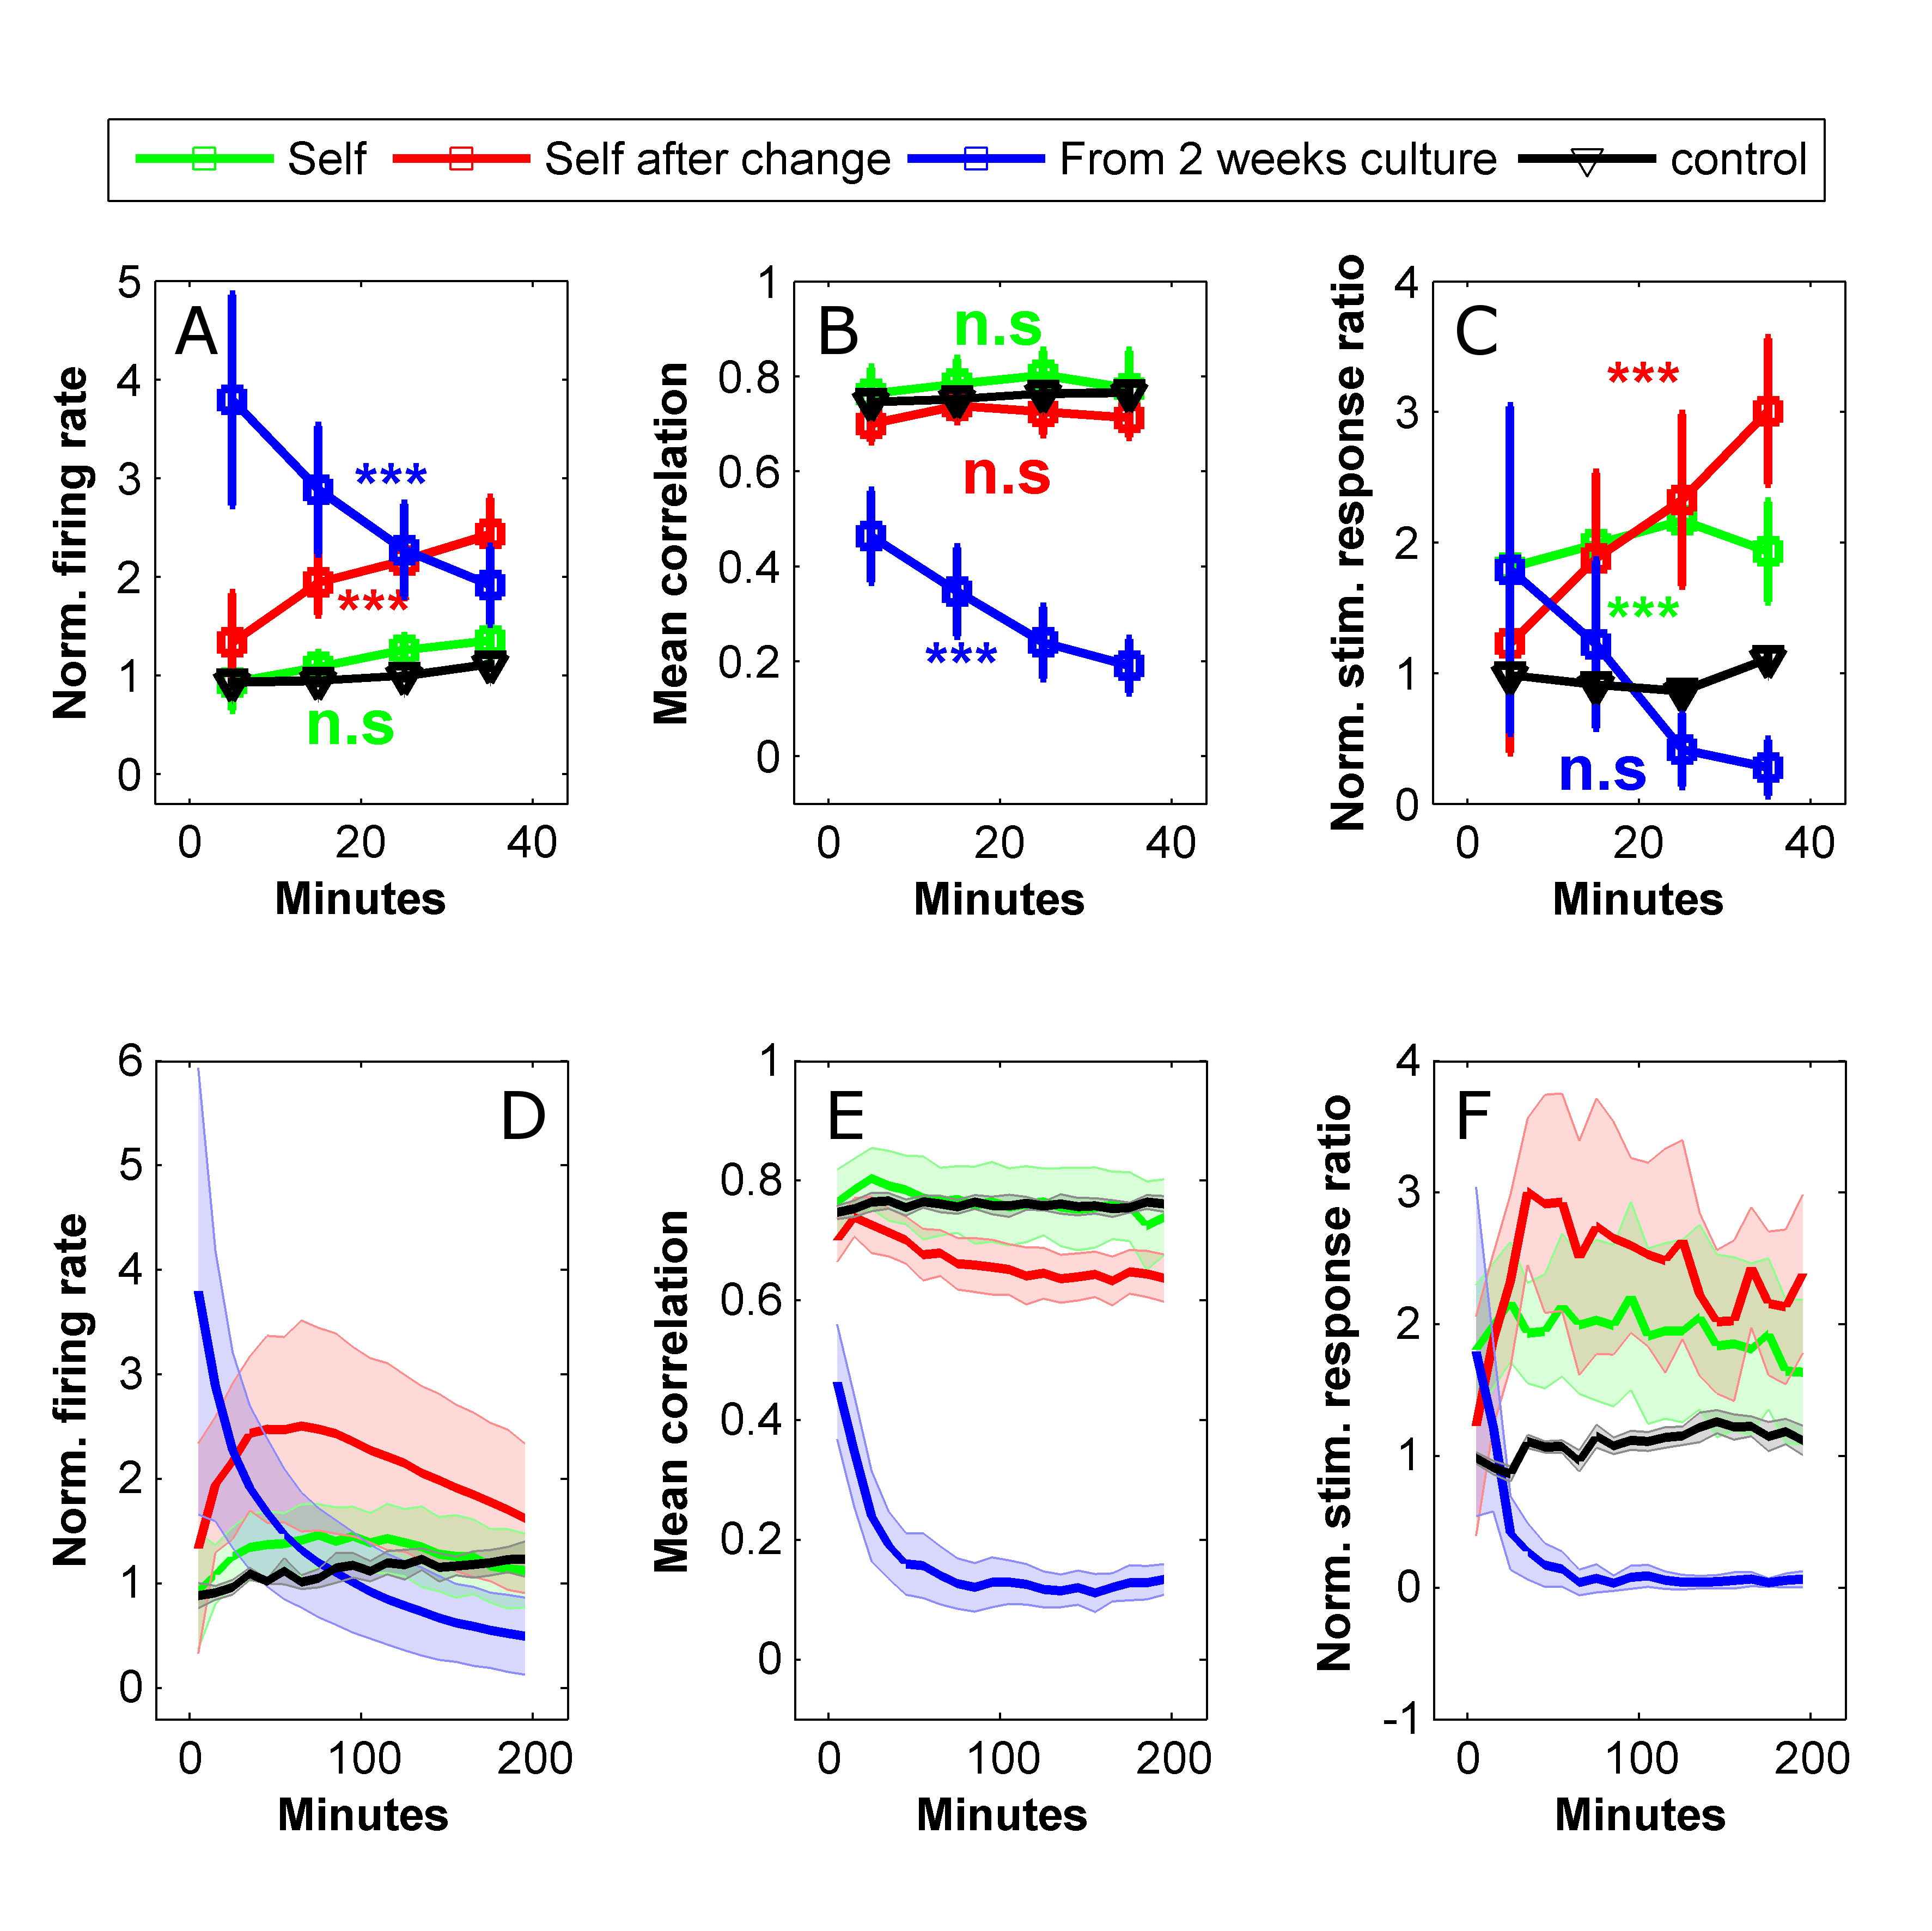
\includegraphics[width=15cm]{chapter5/figures/mediaChangeStats/mediaEffectStats.jpg}
            \caption[Averaged time course of activity measures in old cultures under flow with different media types]{\textbf{The type of media used for flow strongly modulates the activity of the cultures and can cause the activity to crash.} Measures are as in figure \ref{fig:crossFlow:slowFastStats} which also contains further information about the data presentation. Data are based on n=4, 4, 4, 5 experiments for self media, media from young cultures, changed media and control respectively.}

            \label{fig:crossFlow:mediaChangeStats}

        \end{figure}

        Figure \ref{fig:crossFlow:mediaChangeStats} shows the results of flow with the two media types described above. Interestingly, flow with media taken from a young culture (blue curves) resulted in a dramatic disruption to the activity of a similar nature to the one observed in the young cultures, namely that all 3 measures rapidly crashed. However, there were also some obvious differences: Firstly, the total firing rate initially jumped 4-fold and despite dipping rapidly it stayed elevated compared to the control for the first 40 minutes (2-way ANOVA, \(p=5.0\times 10^{-5}\)). In fact, the firing rate decreased to a level lower than control only after about 100 minutes and was never abolished completely. Secondly, the correlation levels were significantly reduced as compared to control immediately with flow onset (2-way ANOVA, \(p=1.0\times 10^{-12}\)) but deteriorated more gradually compared to the young cultures (compare to figure \ref{fig:crossFlow:fastMembraneStats}) and were never completely abolished. Finally, the response to stimulation initially persisted (2-way ANOVA on the first 40 minutes did not reveal a significant difference from control, \(p=0.90\) for group effect and \(0.28\) for interaction effect). However, after 40 minutes the response was already significantly below control (unbalanced t-test on the final sample of panel C, \(p=0.0038\)). This time course of loss of the response to stimulation was slower than in the young cultures where the stimulation response was abolished virtually immediately with the onset of flow.

        Figure \ref{fig:crossFlow:mediaChangeStats} also demonstrates that the mere action of changing the media can significantly affect the the culture's response to flow with this media (red curves). In a 40 minute window after flow initiation this was mainly evident in increase in firing rate as compared to control (2-way ANOVA, \(p=6.5\times 10^{-6}\)) whereas the synchronicity was reduced only with a 90\% level of confidence (2-way ANOVA \(p=0.054\) for group effect). The stimulation response was significantly stronger than control (\(p=7.3\times 10^{-4}\)) but an increase with the same level of confidence was found for the original flow experiment with self media on old cultures. The long term trends show a less stable behaviour under flow with recently changed media in all 3 measures. Nevertheless, the effects of the media change were quite subtle and these culture generally seemed to maintain basic network function under flow and considered useful for experimentation.

        The results provided in this section show that, even in the old cultures, the formulation of the media used for flow is crucial for sustaining a stable network activity. Indeed, as we noted, the old cultures performed better as compared to the young ones but this improvement was marginal given the overall trend. Thus older cultures exhibit a strong sensitivity to the contents of the flow media despite their increased ECM contents and mature synaptic configuration.

        \subsection{How old conditioned media performs on young cultures}
        The results of the previous section suggest that media drawn from old cultures contains chemical species that enable stable network function under flow and that these species are absent in media from young cultures. This led us to ask whether these enabling features of old media are specifically linked to old cultures or are they more universal and would facilitate stable network function under flow for young cultures as well. To answer this question, we conducted a final set of experiments where media taken from old cultures was used for flow on young cultures. Figure \ref{fig:crossFlow:oldOnYoungStats} shows the results of these studies using the same measures used before. Interestingly, old media did in fact improve the performance of young cultures. These cultures generally did not exhibit the high rate tonic firing that characterized cultures under flow with young media (not shown) and indeed the firing rate in the first 40 minutes was not significantly different from control (2-way ANOVA, \(p=0.5\) for group effect). The mean correlation did dip significantly (2-way ANOVA, \(p=0.0016\)) but was initially stable. The stimulation response was also stable but interestingly was significantly \textbf{lower} than the control (2-way ANOVA, \(p=0.0027\)) rather than higher which was the case when the same media was used with old cultures. Nevertheless the longer term performance was unstable as most of the cultures gradually became silenced in the extended period of observation (figure \ref{fig:crossFlow:oldOnYoungStats} D-F). Additionally, it should be noted that these averaged measures are somewhat misleading as the individual measurements in this case were highly variable as could be understood from the thickness of the shaded areas in the extended period panels. Out of 5 cultures measured, 2 had their activity abolished and 3 lost their stimulation response almost immediately. On the other hand, the 2 other culture performed very well under flow. These results demonstrate that the beneficial effects which old conditioned media has on old culture are partially carried over to young cultures. Some of the cultures sustain a stable network activity but only for a short while and in highly variable fashion. These results are not surprising as one might expect that the flow media chemistry needs to match the specific identity and developmental stage of the observed culture.

        \begin{figure}[!htb]
            \centering
            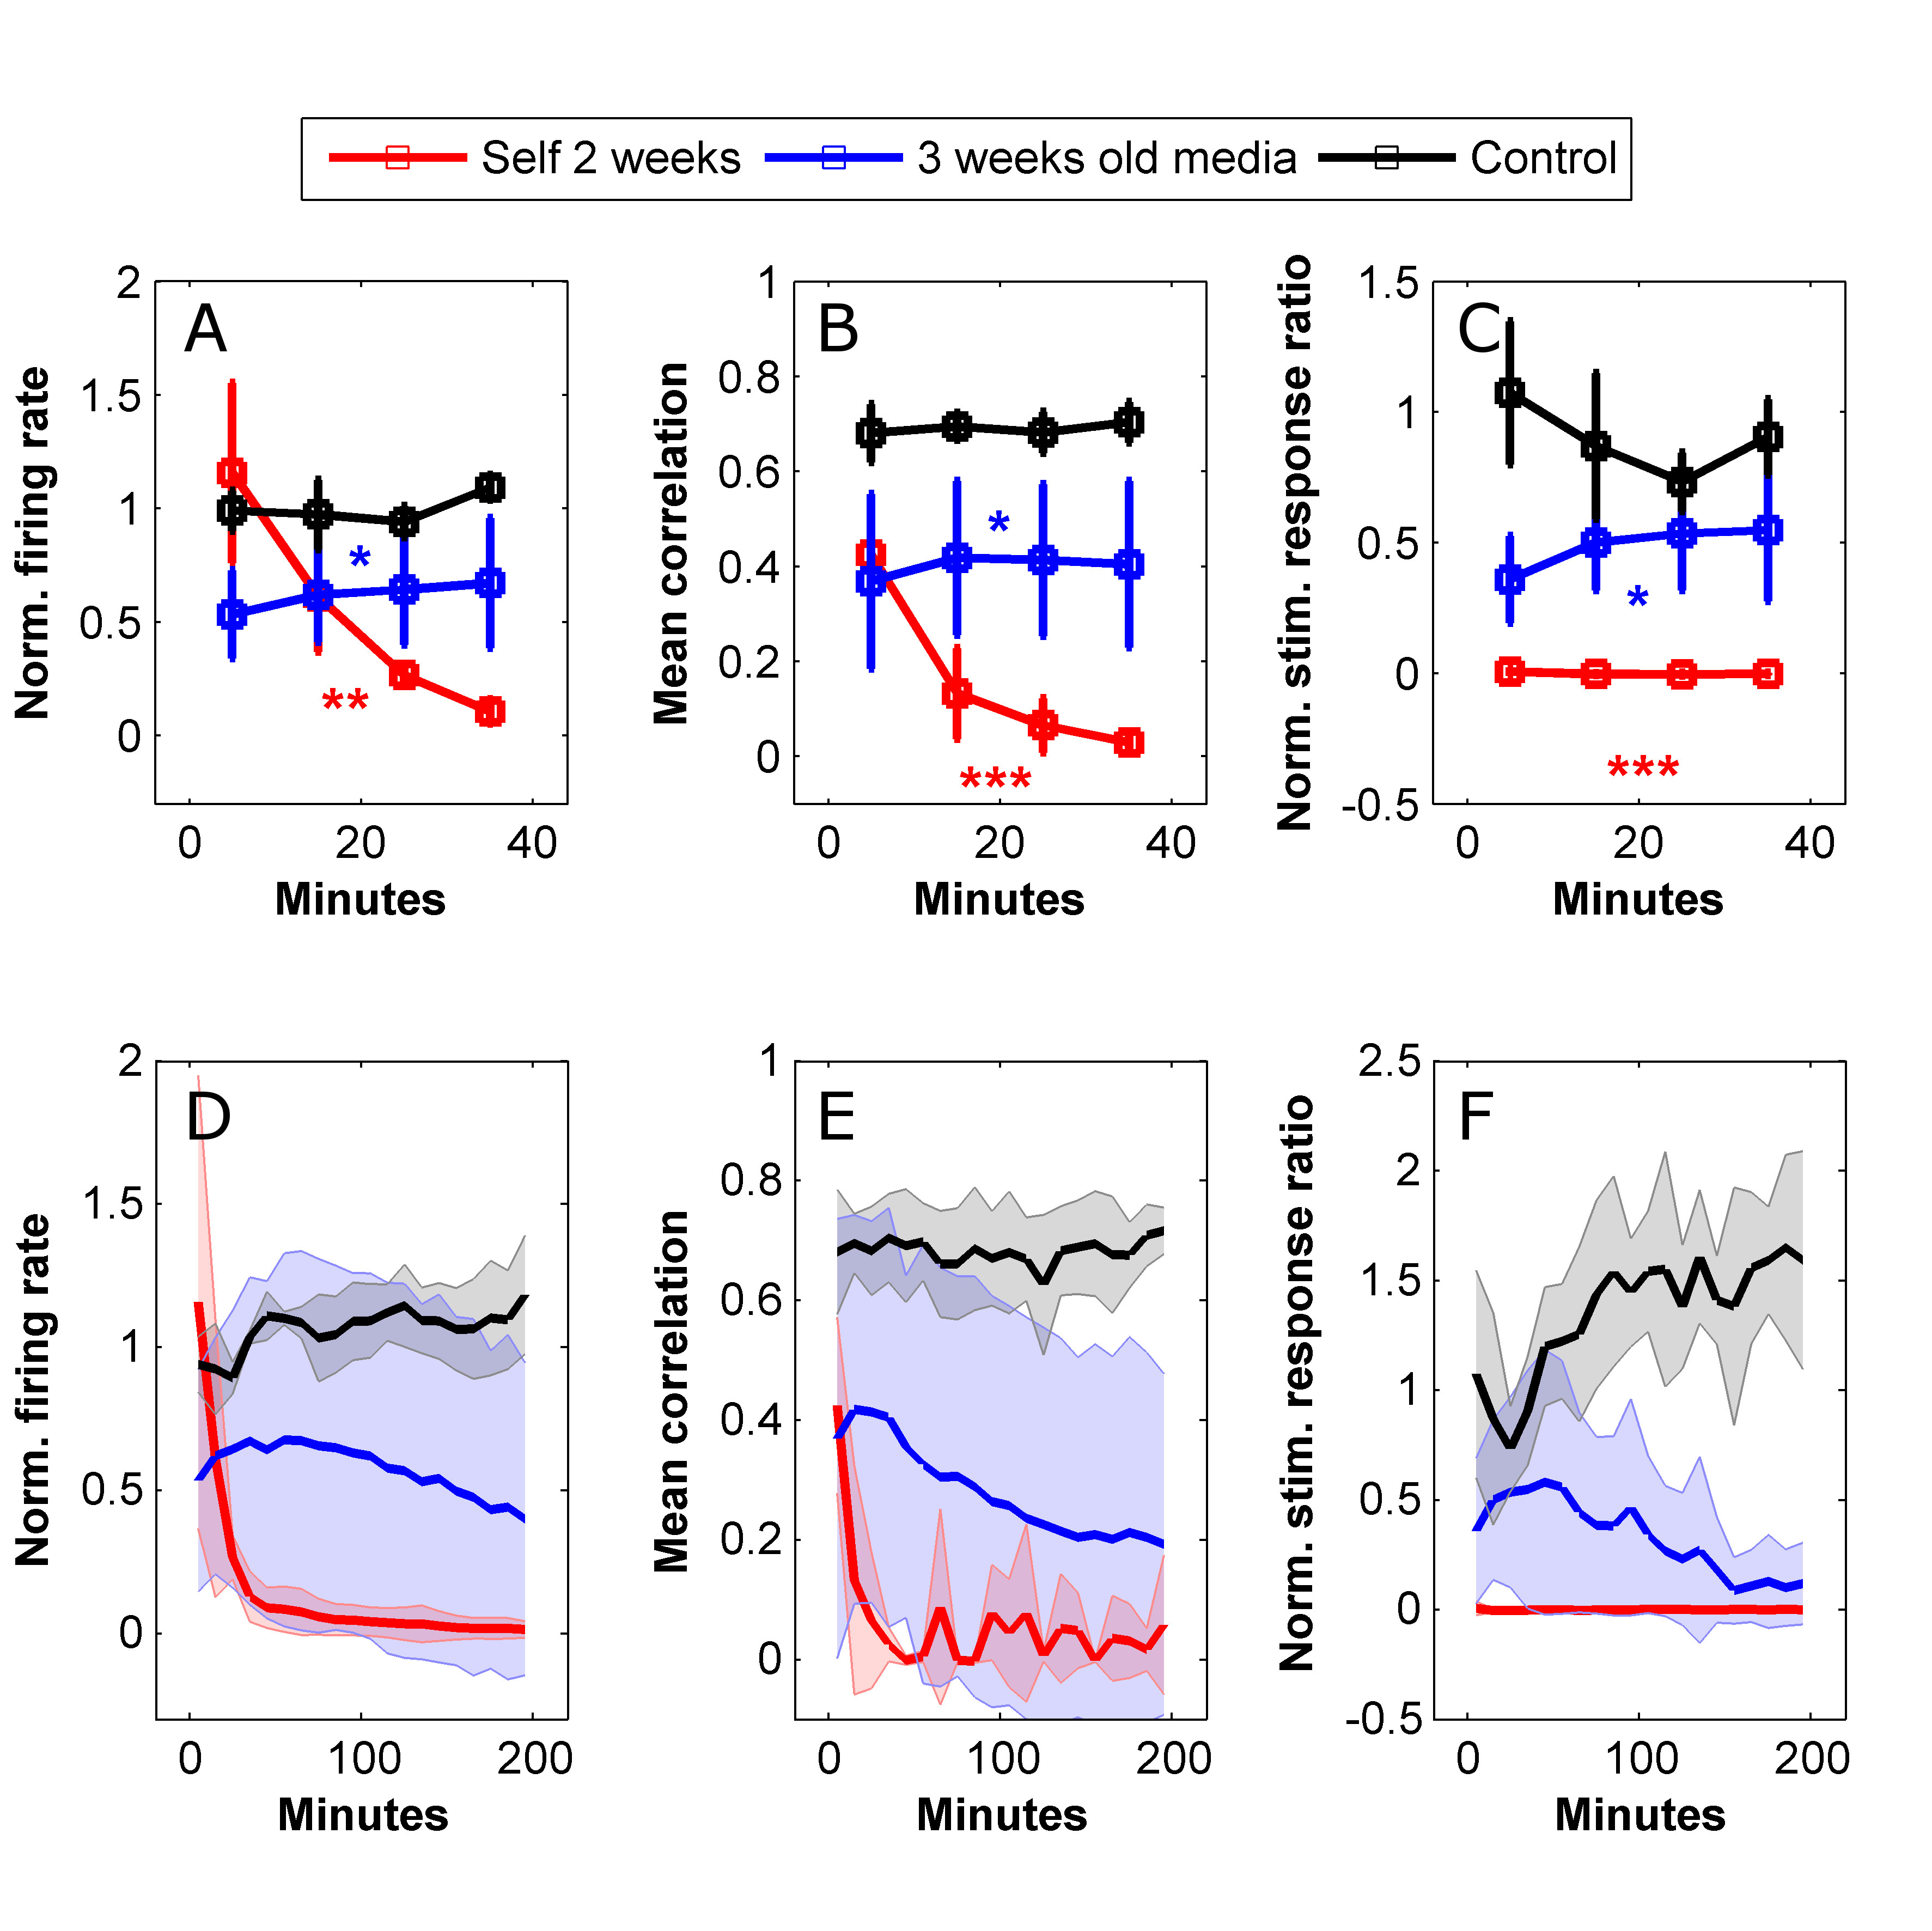
\includegraphics[width=15cm]{chapter5/figures/oldOnYoung/oldOnYoung.jpg}
            \caption[Averaged time course of activity measures in young cultures under flow with old media]{\textbf{Old media improves the performance of young cultures under flow} Measures are as in figure \ref{fig:crossFlow:slowFastStats} which also contains further information about the data presentation. Data are based on n=4, 5, 3 experiments for self media, media from old cultures and control respectively.}
            \label{fig:crossFlow:oldOnYoungStats}
        \end{figure}


\section{Interpretation of the activity under flow results}
\label{sec:crossFlow:interp}
In the previous chapter we have reported that conditioned media can sustain neuronal viability under flow. However, the nature of interaction between the media and culture and cause of the degeneration remained unclear. In this chapter, we extended the flow experiments to observe the network action potential activity under flow and gained valuable insight as to how flow bears on the culture tissue. Previous flow microfluidic work focused on the need of mitigating shear \cite{morel2012amplification,wang2008microfluidics} which neuronal tissue is exposed to and attributed the positive effects of the chemistry of the flow media on the viability to `shear protection' by molecules secreted specifically for that purpose \cite{liu2013galanin}. In this work we observed a strong disruption to the network activity under fast flow. Indeed this could be attributed to shear activating stretch receptors or simply tearing up the cellular membranes and eliciting an inflammatory response. However, using a semi-permeable membrane shown to reduce the shear to negligible levels \cite{morel2012concentration} did not result in any improvement whatsoever. Furthermore, the membrane results were consistent with an assumption that a neuromodulator sized chemical species (\(D=400\frac{\mu m^{2}}{s}\) \cite{johnstoneThesis}) is being diffusively removed through the membrane opening. Calculation based on this scenario predicted that cells located at a distance of \(1-1.5 mm\) from the diffusive sink would be `safe' from the removal. Indeed the shifted recording experiment showed that a culture area partially located in the safe distance maintained its activity with only minor modulation. Had we performed the calculations with diffusive coefficients of ions (\(D=4000\frac{\mu m^{2}}{s}\)) or small proteins  (\(D=40\frac{\mu m^{2}}{s}\)) then we would have expected either a disruption to occur over the entire culture area of the device or no disruption at all, respectively. However, these predictions are in disagreement with the results thus pointing specifically to neurotransmitter sized molecules as the culprits. Given the obvious importance of neurotransmitters to neuronal activity we argue that the immediate activity effects observed here are best explained by action of neurotransmitters on their respective receptor ion channels and that other explanations involving shear should be rejected on the basis of an Occam's Razor reasoning. The results shown in this chapter do not rule out the possibility that shear contributes to other long term effects but they definitely demonstrate a that a disruption to neuronal signalling is a strong part of the effect of flow which  needs to be taken into account.

In section \ref{sec:crossFlow:oldSelf} we showed that the activity in old cultures was maintained under fast flow with self media although these cultures were very sensitive to changes in the media chemistry (for example, their activity was disrupted in similar fashion to what was observed in young cultures, when media from such young cultures was used for flow). This result suggests that self media in old culture is chemically more matched with the micro-environment around the cells than in young cultures. Nevertheless, as the self media is in direct contact with the culture one would expect chemicals secreted by the cells to quickly diffuse to the bulk, especially in the case of small neurotransmitter molecules, so it may seem surprising that a strong gradient would develop between them. However, as mentioned in section \ref{sec:activity:activityStats}, the period of development occurring between the young (beginning of 3\textsuperscript{rd} week) and old age (beginning of 4\textsuperscript{th} week) time frames is characterized by fast changes to the neurotransmission systems. HPLC measurements of the glutamate and GABA contents of neuronal culture media show that the levels of both these major neurotransmitters rise over the first month \textit{in vitro} and saturate only at around day 35 \cite{ramakers1994activity}. In particular, the GABA levels do not rise monotonically but remain low for the first 3 weeks and then jump sharply to reach the final saturated levels. This sharp rise in the media GABA content might correlate with the induction of the astrocytic GABA \cite{lee2010channel} or maturation of late interneurons \cite{hensch2005critical}. Additionally, some reports claim that synaptogenesis in culture extends into the forth week which might also explain the increase in neurotransmitter production during the preceding period \cite{brewer2008neuron,grabrucker2009synaptogenesis}. Although the exact nature and timing of these maturation processes has not been completely clarified, there is ample evidence that the tonic neurotransmitter levels strongly depend on the culture age. In our devices, a large support culture comprising 250k cells is seeded on the outside (compared to 14k inside) and this external culture is probably the main source for diffusible factors in the bulk media. A possible explanation for the mismatch of the self media in young cultures could therefore be that the external support cultures were at a considerably different developmental stage as compared to the internal cultures and so the self media was not well matched to the latter. Indeed it has been shown that cultures grown in microfluidic devices develop faster than standard ones, possibly due to localized buildup of conditioning factors \cite{goyal2011neuronal}. In the case of older devices, which are one week more developed, both the internal and external cultures may have entered a saturation in development so they were more similar. Another possible explanation for the self media mismatch is that during periods of accelerated development the rate of changes to the local neurotransmitter environment exceeds the rate of diffusion so that the bulk media is `lagging behind' in accumulating the chemicals from the microenvironment. After all, even though neurotransmitters are small molecules they would take about 17 hours to diffuse through a media reservoir of height \(10 mm\) (note that the bulk media volume per sample was bigger in the cross flow devices to allow enough supply for the flow session).

The afore-mentioned delay in development of some GABAergic elements of the neurotransmission system raises the possibility that it is indeed GABA that is lacking in the flow media. Indeed it has been shown that the action of tonic extrasynaptic GABA exerts inhibition that is several times \textbf{stronger} than that of the fast synaptic one \cite{farrant2005variations,mody2004diversity} which could explain how drastic the effects of flow are. Some specific features in the response to flow provide further indication that an inhibitory transmitter is involved. Namely, when young media was used on old cultures the response was an immediate 4 fold increase in the spiking activity followed by a gradual decay, possibly due to depletion of resources. This could be interpreted as a release from strong inhibition. On the other hand, when old media was used on young cultures the stimulation response immediately decreased and the activity was silenced after a while. This could be explained by the young cultures being accustomed to lower levels of tonic inhibitor compared to the old cultures and hence becoming silent when exposed to media from the latter. Indeed GABA is recognized as the major inhibitory neurotransmitter operating in the CNS and its extrasynaptic function has been receiving growing interest \cite{mody2004diversity,lee2010channel,olah2009regulation}. Nevertheless, the activity patterns observed under fast flow with young conditioned media are inconsistent with results from application of GABA antagonists \cite{bikbaev2015brain,li2007long}. These studies did not report a decrease in synchronization but rather an increase in burst frequency and burst length so removal of GABA alone is probably not enough to explain the observed disturbance. Intrinsic volume transmission comprises an assortment of other signals including the major excitatory neurotransmitter glutamate \cite{cavelier2005tonic} as well as adenosine \cite{wall2015localized}, ATP, NO and various neuropeptides \cite{fuxe2010discovery,taber2014volume}. Thus the observed disturbance cannot be attributed to any specific species and is more likely a holistic effect associated with perturbations to all the intrinsic volume transmission processes at varying degrees. We believe that our results warrant an in depth investigation into the source of the disruption as it could entail a novel signalling species. Such an investigation could proceed by applying a cocktail of receptor blockers matching the known volume transmission signals to see if the effects of flow may be reproduced in this manner.

Even when the media is matched the flow could still affect more than just the extrasynaptic tonic concentrations of signalling molecules. This is explained next.  The accepted paradigm is that neurotransmission proceeds in two distinct compartments, intra- and extra-synaptic. The most recognized neurotransmission action is the fast synaptic one where vesicle release on the presynaptic side causes an extremely rapid (time constant \(<1ms\)) phasic increase in the neurotransmitter content in the synaptic cleft. The time course of these phasic signals is mainly determined by outwards diffusion to the extrasynaptic space \cite{clements1996transmitter}. Although the phasic dynamics are the hallmark of synaptic function it has also been established that there is an appreciable tonic concentration of neurotransmitters in the synaptic cleft which is enough for a continuous activation of postsynaptic receptors \cite{sah1989tonic}. The source of this tonic transmitter level is most probably simply diffusion from the extrasynaptic space. In contrast to the intrasynaptic compartment where only neurotransmitters are known to operate, the extrasynaptic compartment contains a mixture of neurotransmitters and neuromodulators operating through both ionotropic and metabotropic receptors. In recent years, more focus has been given to the extrasynaptic species which were shown to have a strong effect on network dynamics and therefore a computational importance \cite{wall2015localized,mann2010control,hamann2002tonic,lenk2016understanding,cavelier2005tonic}. Such extrasynaptic neurotransmitters and neuromodulators are usually referred to as the 'tonic environment'. However, this terminology could be misleading by giving the impression that this environment is completely static whereas in fact it is temporally varying (i.e., it has phasic aspects) or else it would not be able to modulate the network activity. Since this intrinsic volume transmission is based on discrete secretion events from specific cells it stands to reason that it will have a spatial organization as well (this was shown for the case of adenosine in \cite{wall2015localized}). Thus, to summarize, both intra- and extra-synaptic compartments contain signals with tonic and phasic components and they are not completely segregated but rather coupled via diffusion (e.g., synaptic spill over contributes to the phasic extrasynaptic signals and changes to extrasynaptic concentrations of non-synaptic origins can influence the tonic activation of the synapses).

\begin{wrapfigure}{r}{5cm}
      \centering
      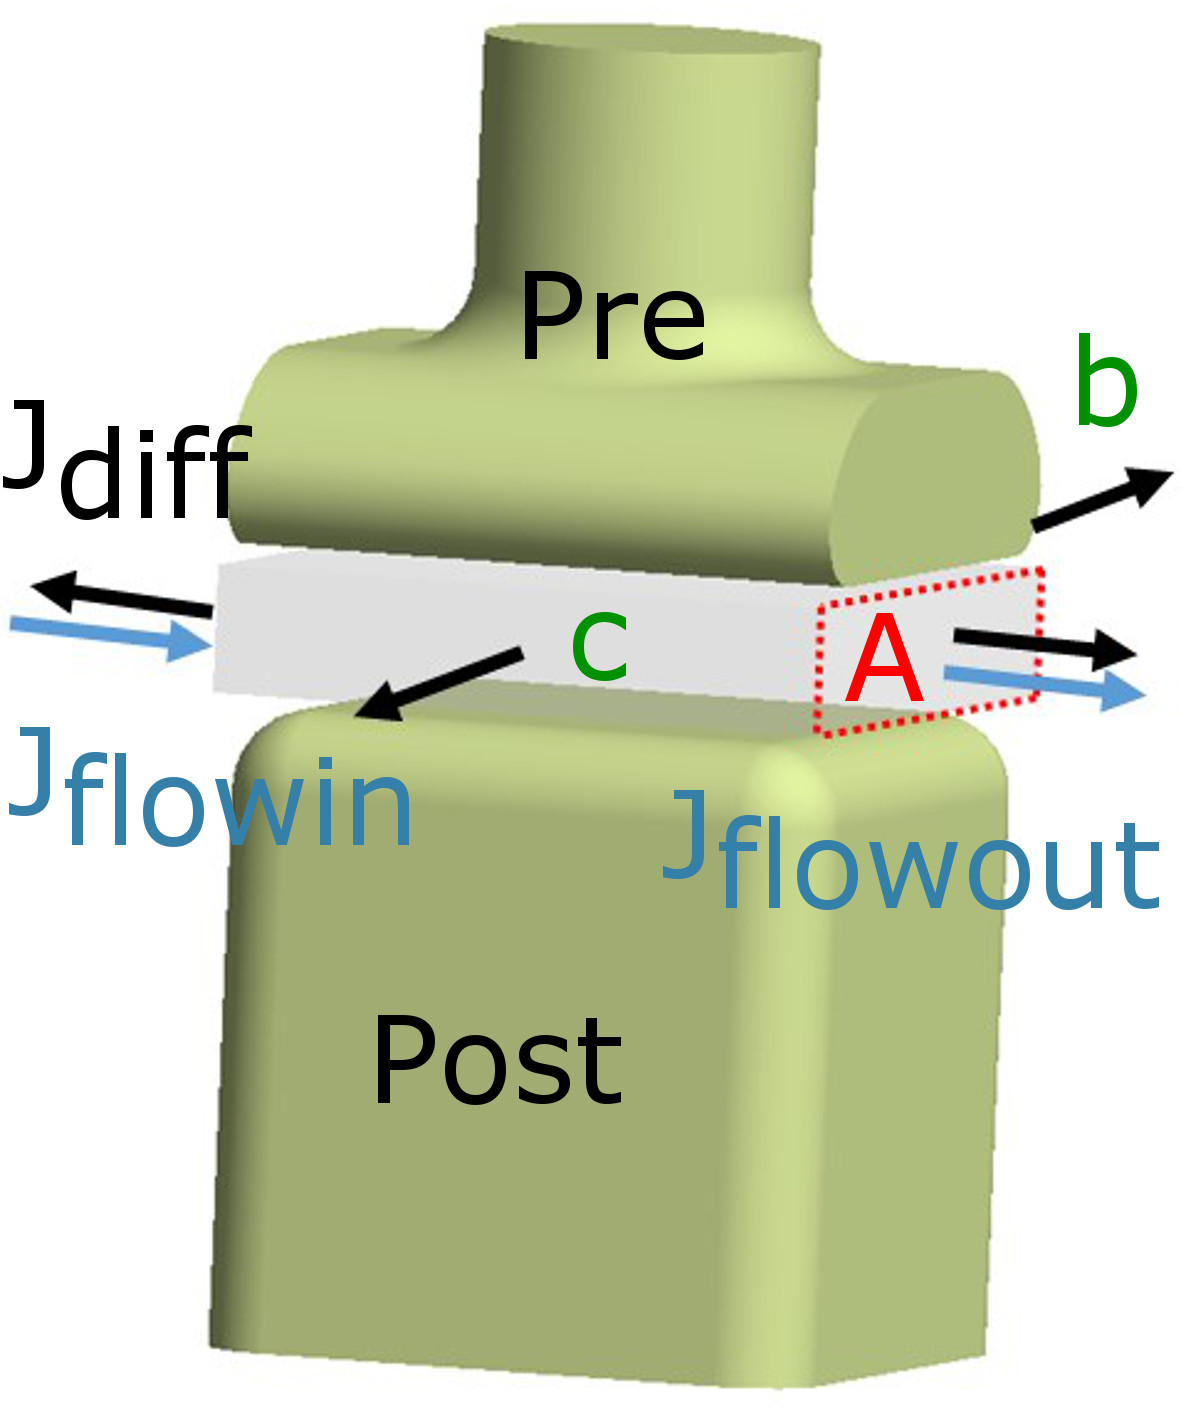
\includegraphics[width=5cm]{chapter5/figures/synapse/synapseIllustration.jpg}
      \caption[Illustration of a synaptic cleft with flow running through it]{Illustration of the synaptic cleft geometry and symbols used to compare the convective and diffusive flux in the case where the flow runs directly through the synapse.}
      \label{fig:crossFlow:synapse}
\end{wrapfigure}

Out of the signalling modes mentioned above, The phasic synaptic one is the least likely to be affected by the flow because the neurotransmitter pulses are extremely quick and the concentrations are dependent on release from vesicles which are located intracellularly. Nevertheless there is a concern that if rapid convective flow is channeled through the synaptic cleft then it could wash away the neurotransmitter molecules as they are released and therefore to significantly modify the temporal profile of activation. To check if this could indeed be of concern we compared the diffusive flux out of a synapse with the expected convective flux due to flow assuming that the synapse is indeed open and that the flow is directed perpendicularly to the transmission line as depicted in figure \ref{fig:crossFlow:synapse}. The calculations are as follows: assuming a parabolic flow profile the flow velocity around the synapses is \[u=u_{avg}(1-\frac{y^{2}}{h^{2}})\approx 15\frac{\mu m}{s}\] where \(u_{avg}=200\frac{\mu m}{s}\) is the average flow velocity, \(h=50\mu m\) is half the channel height and \(y=48\mu m\) is the location of the synapses relative to the horizontal center of the channel, i.e., \(2\mu m\) from the surface. The diffusive flux out of the synapse is \[J_{diff}=D\frac{c-b}{d}(4A)\approx 32(c-b)\frac{moles}{s}\] where \(D=400\frac{\mu m^{2}}{s}\) is the diffusion coefficient for a neurotransmitter sized molecule in free media, \(c\) and \(b\) are the intra- and extra-synaptic neurotransmitter concentrations, respectively in \(\frac{moles}{\mu m^{3}}\), \(d=0.2\mu m\) is the diffusion distance and \(A=0.2\times 0.02=0.004\mu m^{2}\) is the area of one external face of the synaptic cleft (taking the cleft gap to be \(0.02\mu m\) and cleft width to be \(0.2\mu m\)) (\(4A\) is then the entire face area available for diffusion). The total convective flux is \[J_{conv}=J_{flowout}-J_{flowin}=Auc-Aub=Au(c-b)=0.06(c-b)\frac{moles}{s}.\] Thus, somewhat un-intuitively and owing to its nano-scale dimensions, the outwards flux out of the cleft due to diffusion (which is the main determinant of the temporal concentration profile during synaptic activation \cite{clements1996transmitter}) is 3 orders of magnitude larger than the that due to convection even if the cleft is completely open to the flow. In reality, the synapses are usually enveloped in neuronal and astrocytic membranes which are unlikely to allow any degree of flow through. Thus we would expect phasic synaptic dynamics to be maintained even under much faster flow rates or shallow device geometries (i.e., where the flow velocity at the boundaries would be higher). However, the same cannot be said about the phasic extrasynaptic signalling which is much slower and operates over much larger space scales and about tonic synaptic concentrations. Thus, fast flow, beyond the obvious effect of changing the basal extrasynaptic species concentrations, could have generated the observed disruptions by indirectly changing the tonic receptor activation within the synapses and also by disturbing the phasic (and spatially organized) aspects of the intrinsic volume transmission.




\section{Chapter conclusion}
We have argued that the fast microfluidic flow operates as a 'concentration clamp' because it delivers chemical species faster than the culture can uptake or metabolize. This claim has not been fully tested here and doing so might require use of biosensors to directly measure some of the extrasynaptic species. Nevertheless, if this is indeed the case, we propose that, apart from the obvious rapid agonist delivery application, rapid microfluidic flow offers a novel way of holding extrasynaptic concentrations of signalling molecules at set levels. Since neuroactive chemical like neurotransmitters and neuromodulators are directly controlled by the tissue, applying them to the bath is ineffective so the study of their function is classically performed via pharmacology to block the associated receptors. However, this approach ignores potential indirect effects of the presence of these agonists, e.g., elevated extrasynaptic glutamate may operate both through extrasynaptic metabotropic receptors as well as through tonic activation of excitatory synapses. Thus it would be beneficial to be able to control the extracellular concentration of the chemicals to check for remaining effects beyond the obvious receptor blockade. Indeed direct control over extracellular concentration is made possible through enzymatic degradation or chelating agents (e.g., \cite{wall2002furosemide}) but that approach is less accurate and depends on availability of specific pharmacology. Thus the so called concentration clamp offers a method of holding an entire tissue at a specific concentration. Additionally, by applying the rapid agonist delivery approach, one could artificially generate volume transmission pulses of specific agonists while keeping others at a constant level. This would require adaptation of the microfluidic geometry and application paradigm to the required time scales but offers a novel way of studying intrinsic volume transmission processes in neural tissue.

Finally, The control experiments presented in this chapter and in section \ref{sec:devices:viabilityAssay} suggested that the imposed 'concentration clamp' is the main culprit in the observed effects of flow, both in terms of activity as well as viability. Because of the strong action of diffusion at short distances the only way to restore volume transmission processes that are perturbed by the flow is to increase the distance to the flow interface. This may have implications on the level of functionality and viability that may be achieved while preserving the time scales of the drug delivery.

Nevertheless, we have identified conditioned where the network activity is adequately maintained under fast flow. The flow protocol described in this chapter will be the basis for the final phasic neuromodulatory signalling system described in the next (and final) chapter.
